\section{Event Topology and Spherical Harmonics Analysis}
\label{sec:topology_and_harmonics}

\subsection{Topology of 0\nbb-decay and \B~Events}
\label{subsec:topology}
%Signature of the 0\nbb-decay is two electrons with total kinetic energy equal to the isotope Q-value (e.g., 2.529~MeV for $\Te$). Therefore all \B-decay searches are designed to look for an excess of events in the energy spectrum around Q-value over the predicted number of background events. Backgrounds suc0\nbbh as \B solar neutrinos have distinct event topology that can be used to improve experimental sensitivity to the the 0\nbb-decay signal.

For all isotopes considered for searches of 0\nbb-decay, the electrons emitted by the process with energies around the Q-value will be above Cherenkov threshold in liquid scintillators.  Each electron above the threshold will produce a fuzzy ring of Cherenkov light at the detector surface. The fuzziness of the ring depends on electron scattering. In most cases Cherenkov rings from low energy electrons degrade to randomly shaped clusters of Cherenkov photons around the direction of the electron track. 

A large fraction of 0\nbb-decay events will have two Cherenkov clusters~\footnote{Only one Cherenkov cluster is produced when either the angle between the two 0\nbb-decay electrons is too small or when the energy splits between the electrons in such a way that one electron falls below the Cherenkov threshold.} as opposed to one cluster from \B events. Therefore, accurately distinguishing between a 0\nbb-decay signal from a \B background event depends on the ability to identify the topology of Cherenkov light on the detector sphere on top of uniformly distributed scintillation light. We show that an analysis of spherical harmonics on the spatial distribution of early photons can be used to separate 0\nbb-decay and from \B events.


In order to illustrate differences between different event topologies, we introduce three example event topologies: two electrons produced back-to-back at an 180$^{\circ}$ angle, two electrons at a 90$^{\circ}$ angle, and a single electron. The first two are representative of topologies for 0\nbb-decay signal events while the latter is representative of \B background events. Figure~\ref{fig:Display_top_5MeV} shows the Cherenkov photon distributions of 5~MeV electrons for each of the three topologies. Each distribution is made by overlaying 100 events in order to make the Cherenkov rings more visible. Note that in this overlay, we assume a quantum efficiency (QE) of one for the photodetectors.

\begin{figure*}[h]
  \centering
  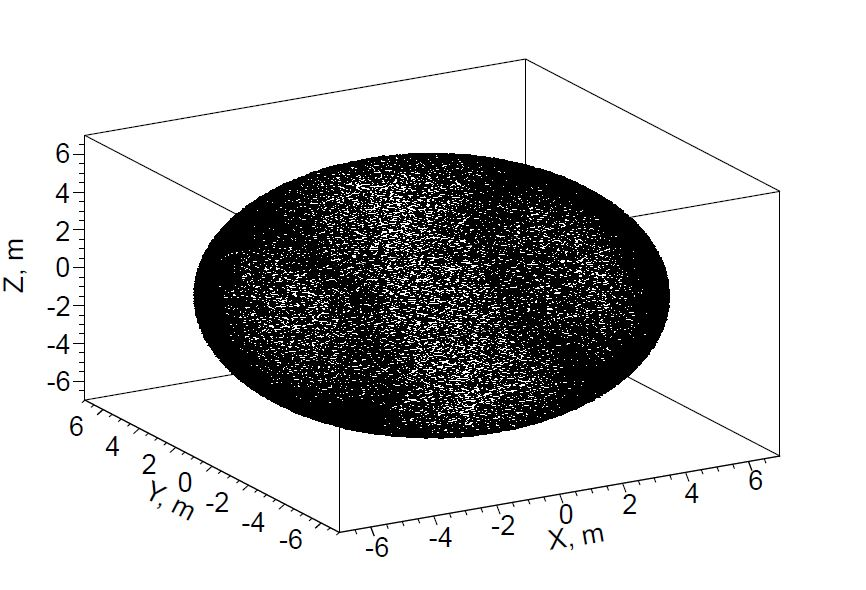
\includegraphics[width=0.3\textwidth]{hDisplay_topology180_5MeV.JPG}
  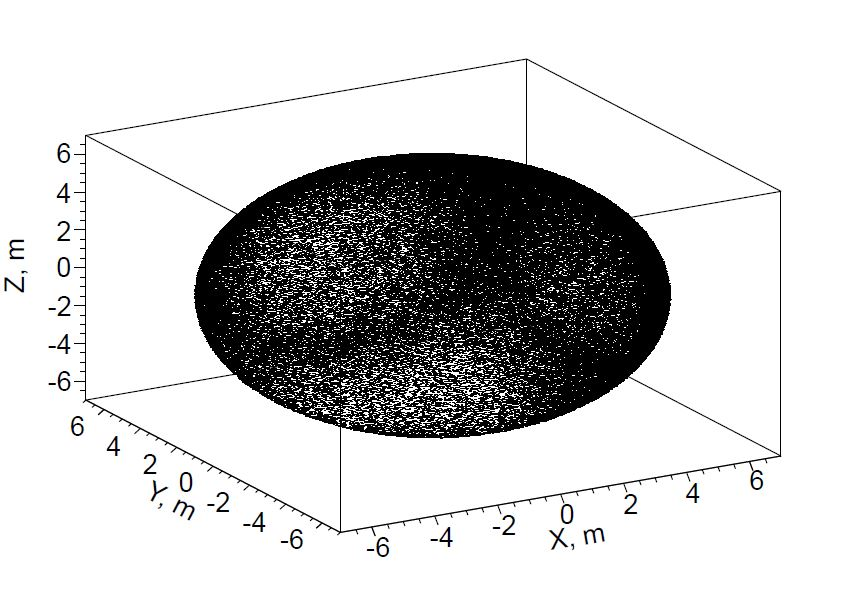
\includegraphics[width=0.3\textwidth]{hDisplay_topology90_5MeV.JPG}
  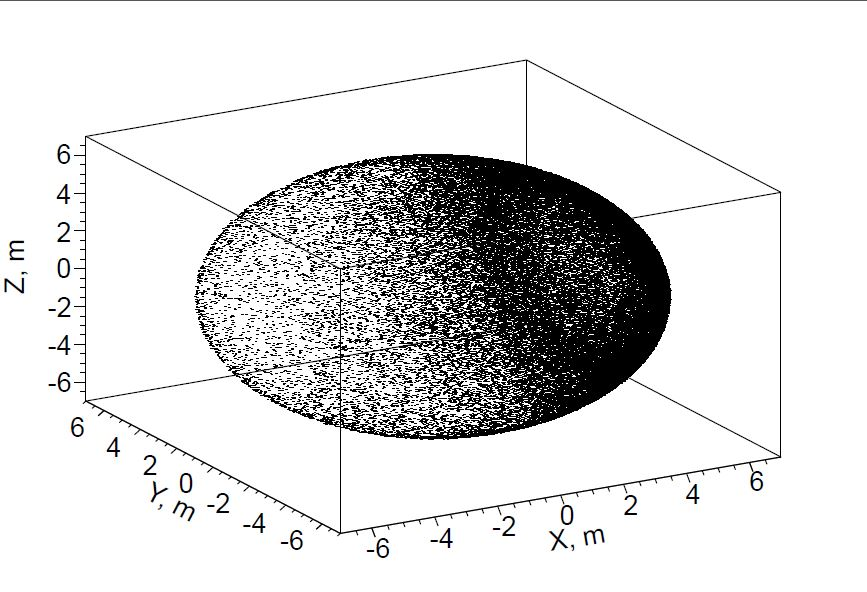
\includegraphics[width=0.3\textwidth]{hDisplay_1el_5MeV.JPG}
  \caption{Cherenkov photons distributions on the detector sphere for
    the three representative event topologies: two back-to-back
    electrons (\emph{left}), two electrons at 90$^{\circ}$ angle
    (\emph{middle}), and a single electron (\emph{center}).  All
    electrons are 5~MeV and originate at the center of the
    detector. 100 events overlayed for better visibility of the
    Cherenkov rings. 100\% QE is assumed. \JOcom{These can not be
      included as PDFs, but my conversion shrunk the size.}}
  \label{fig:Display_top_5MeV}
\end{figure*}


\begin{figure*}[h]
  \centering
  \begin{tabular}{c c c}
  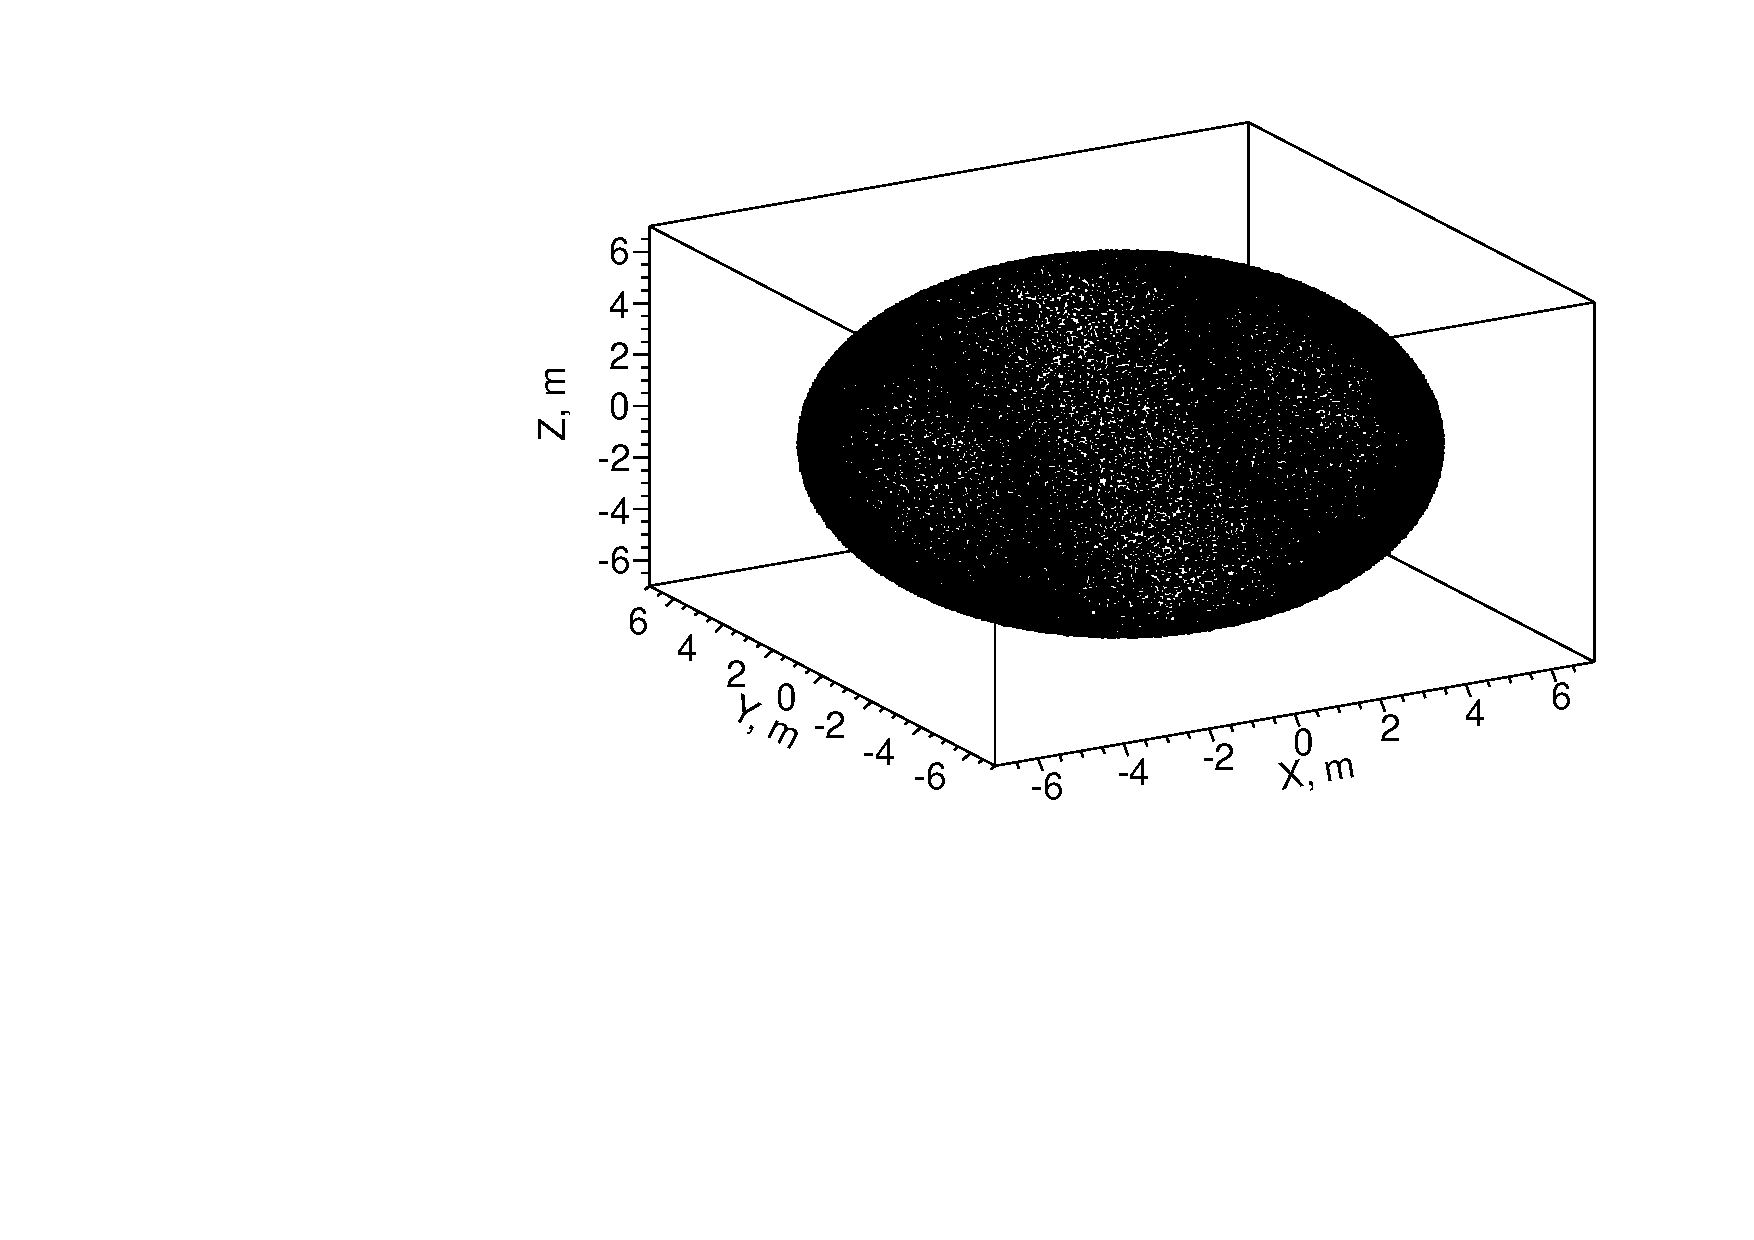
\includegraphics[width=0.3\textwidth]{hDisplay_topology180_5MeV.pdf} &
  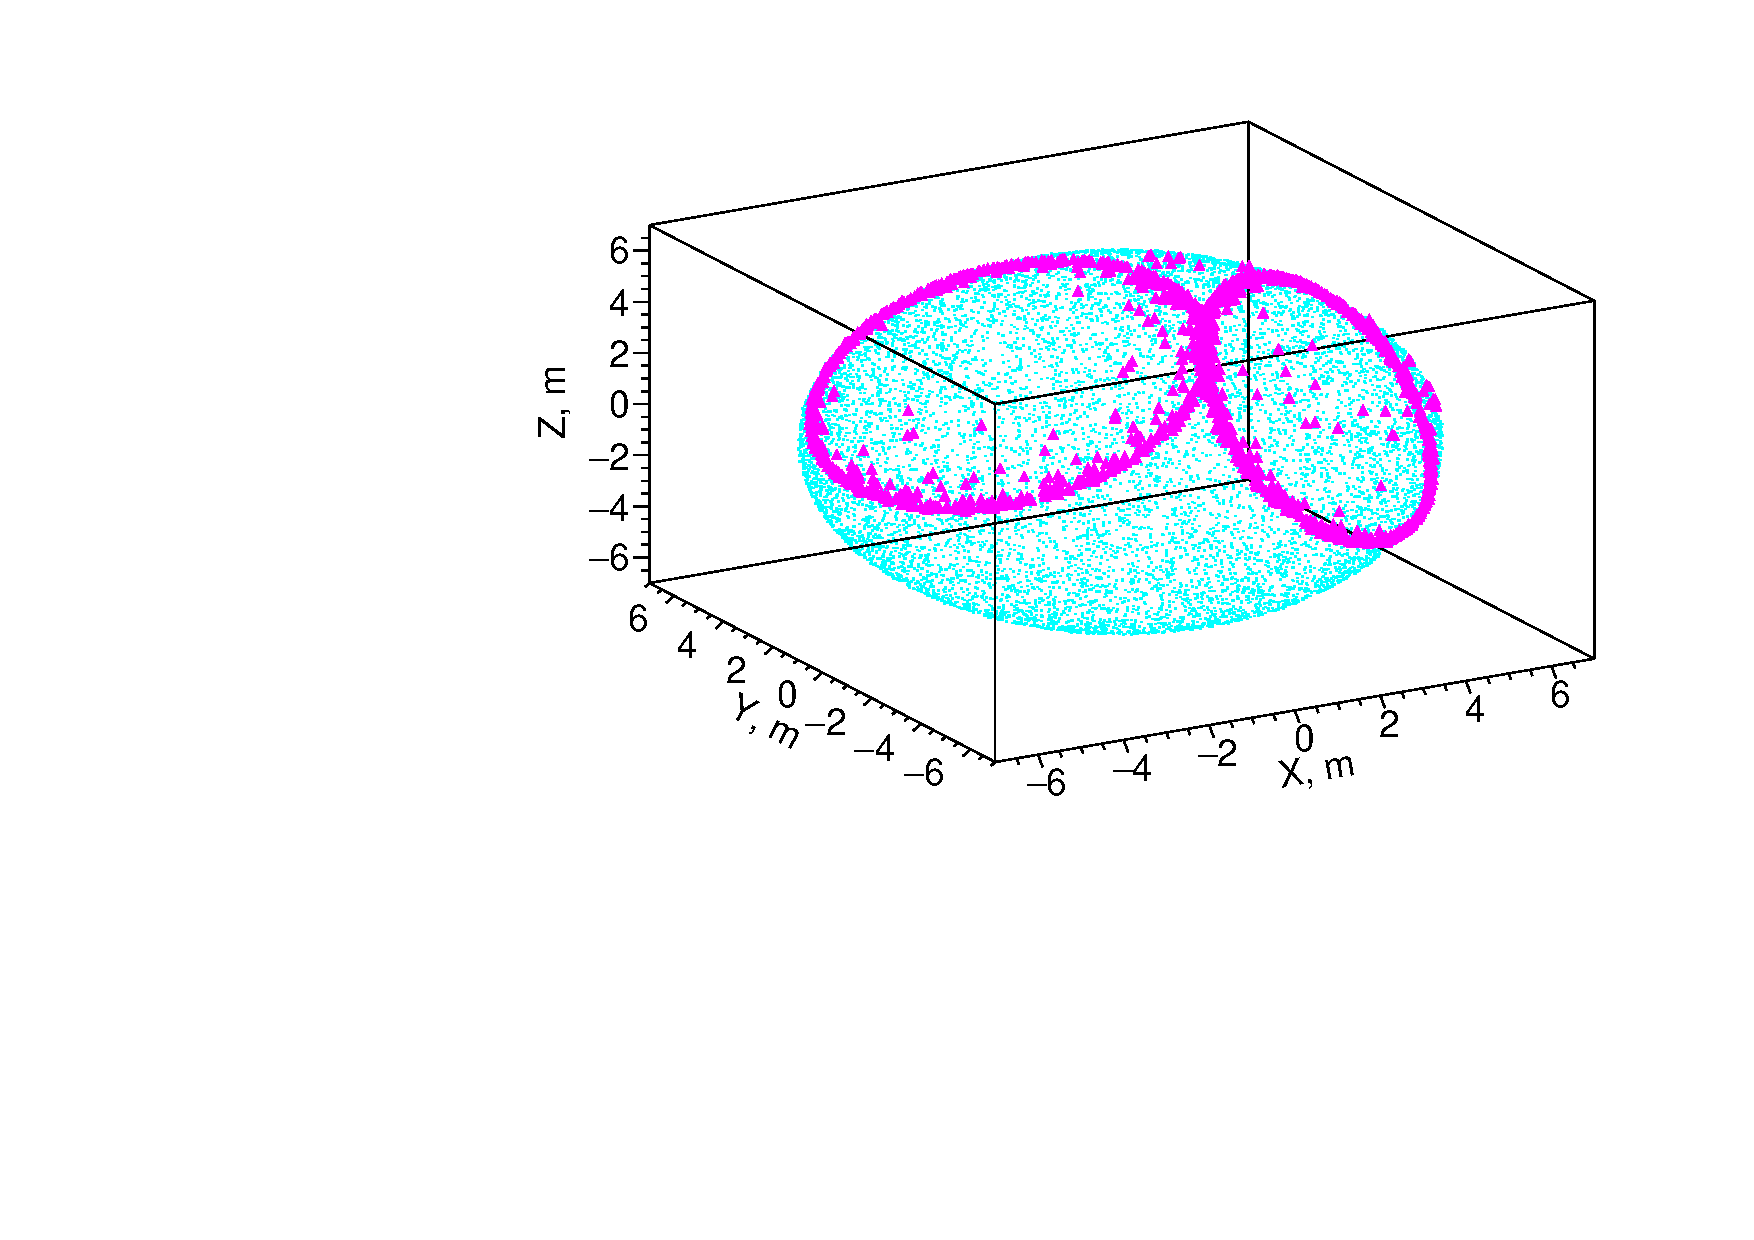
\includegraphics[width=0.3\textwidth]{hDisplay_topology90_5MeV.pdf} &
  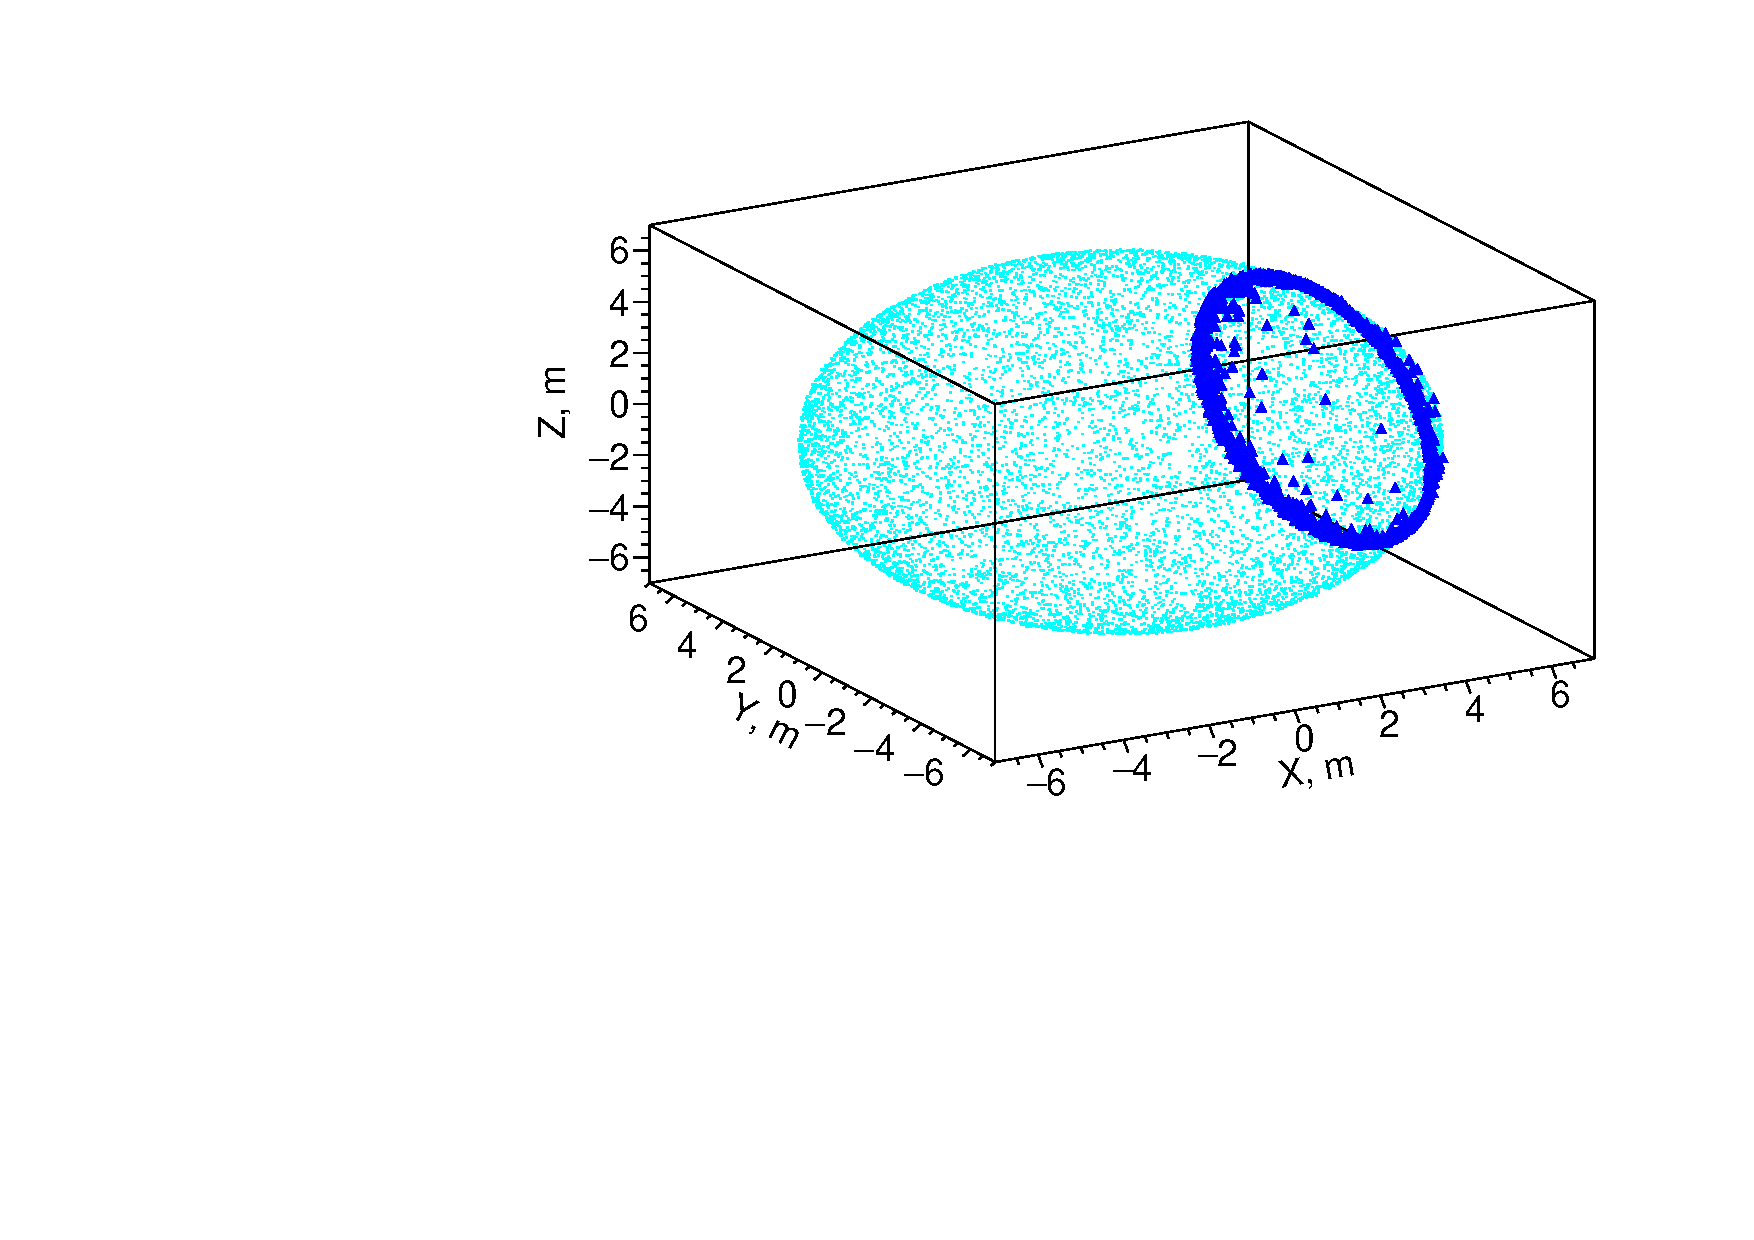
\includegraphics[width=0.3\textwidth]{hDisplay_1el_10MeV.pdf} \\
  \end{tabular}
  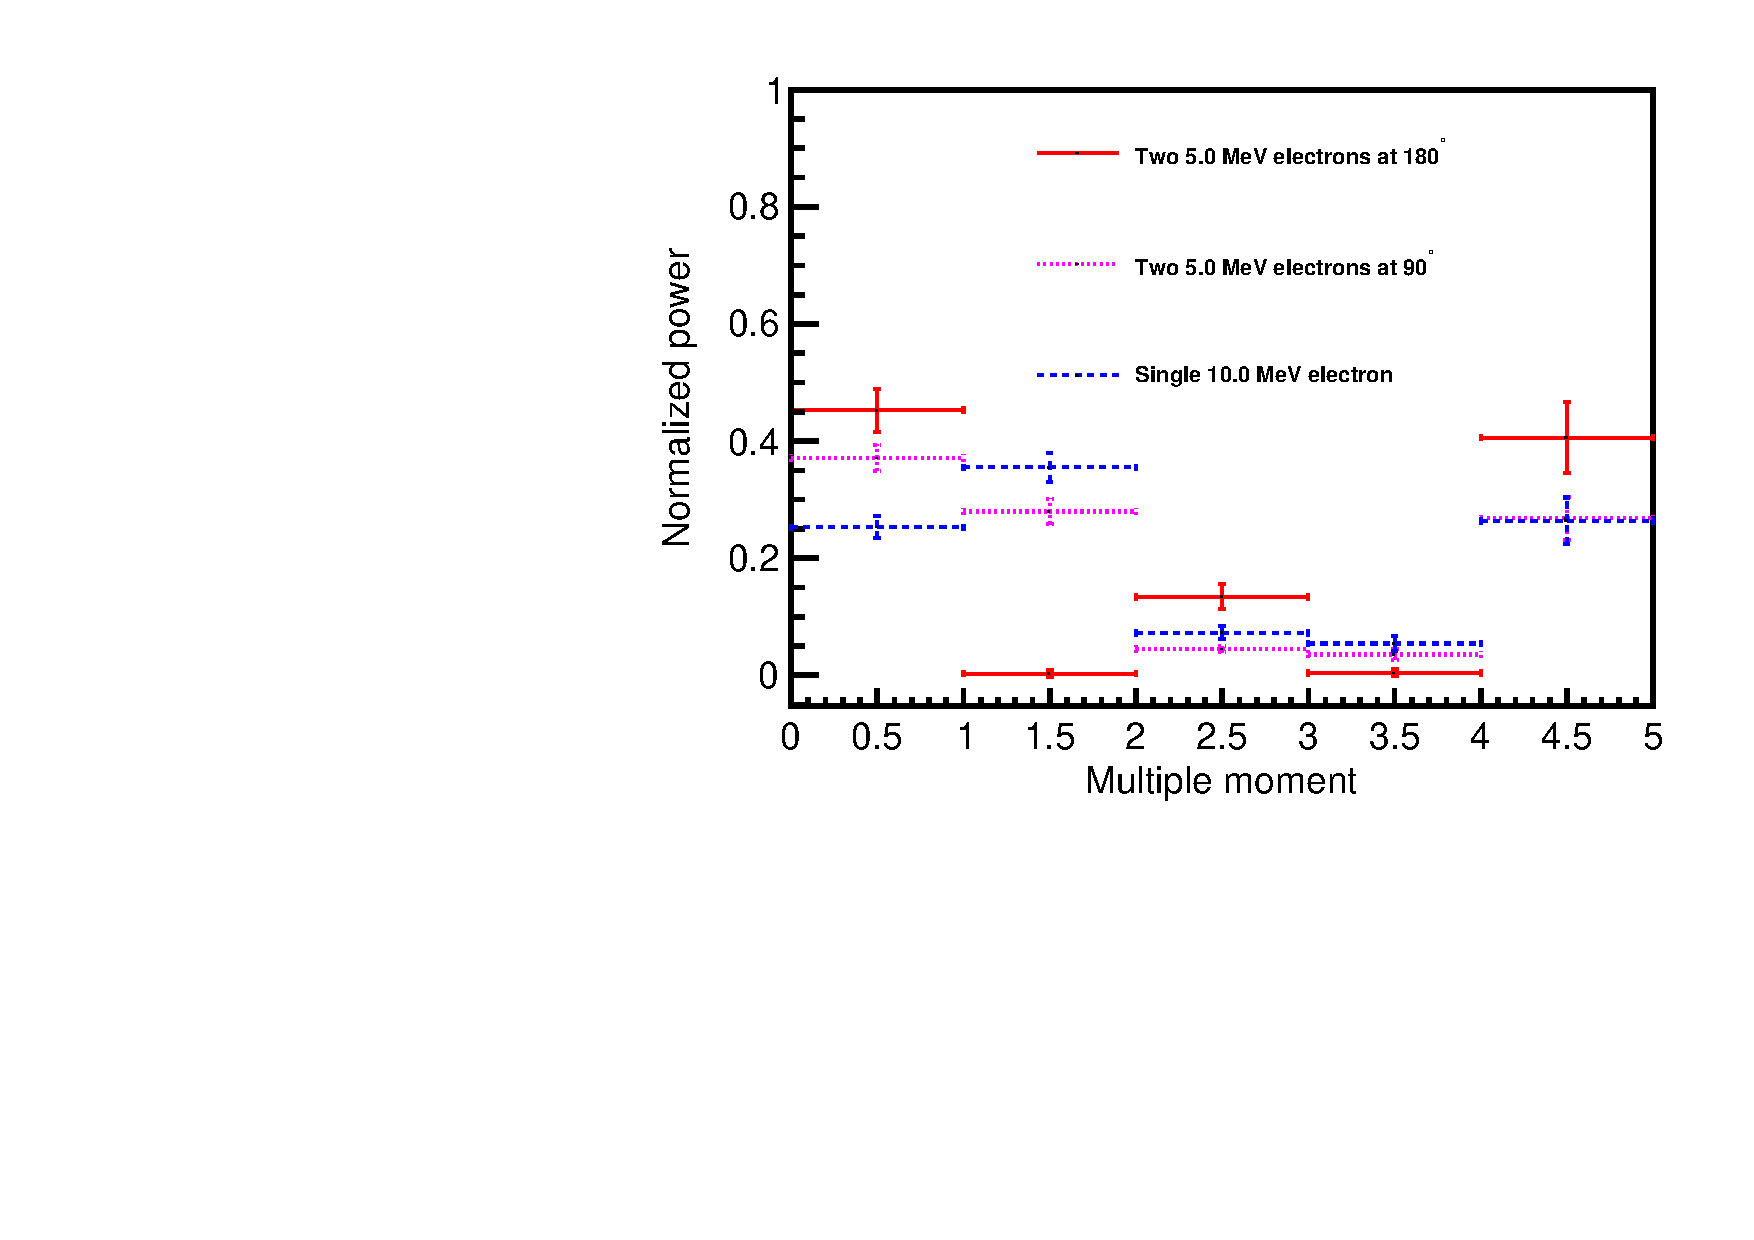
\includegraphics[width=0.9\textwidth]{hMultipleMoment_CHELight_VtxSmear0cm_VtxShiftX0cm_999p9ns_5p0MeV_center_NoMultScat.pdf}
  \caption{CCherenkov photons distributions on the detector sphere for
    the three representative event topologies: two back-to-back
    electrons (\emph{left}), two electrons at 90$^{\circ}$ angle
    (\emph{middle}), and a single electron (\emph{center}).  All
    electrons are 5~MeV and originate at the center of the
    detector. 100 events overlayed for better visibility of the
    Cherenkov rings. 100\% QE is assumed. \JOcom{These can not be
      included as PDFs, but my conversion shrunk the size.}}
  \label{fig:Event_Topology}
\end{figure*}

In practice, Cherenkov rings from low energy electrons are not clearly visible. Examples of such Cherenkov clusters, produced by events with a total kinetic energy of 2.539~MeV (the Q-value of \Te), are shown in Fig.~\ref{fig:Display_top_2p5MeV}. One can try to guess the event topology by comparing different segments of the detector sphere.

\begin{figure*}[h]
  \centering
  \begin{tabular}{c c c}
  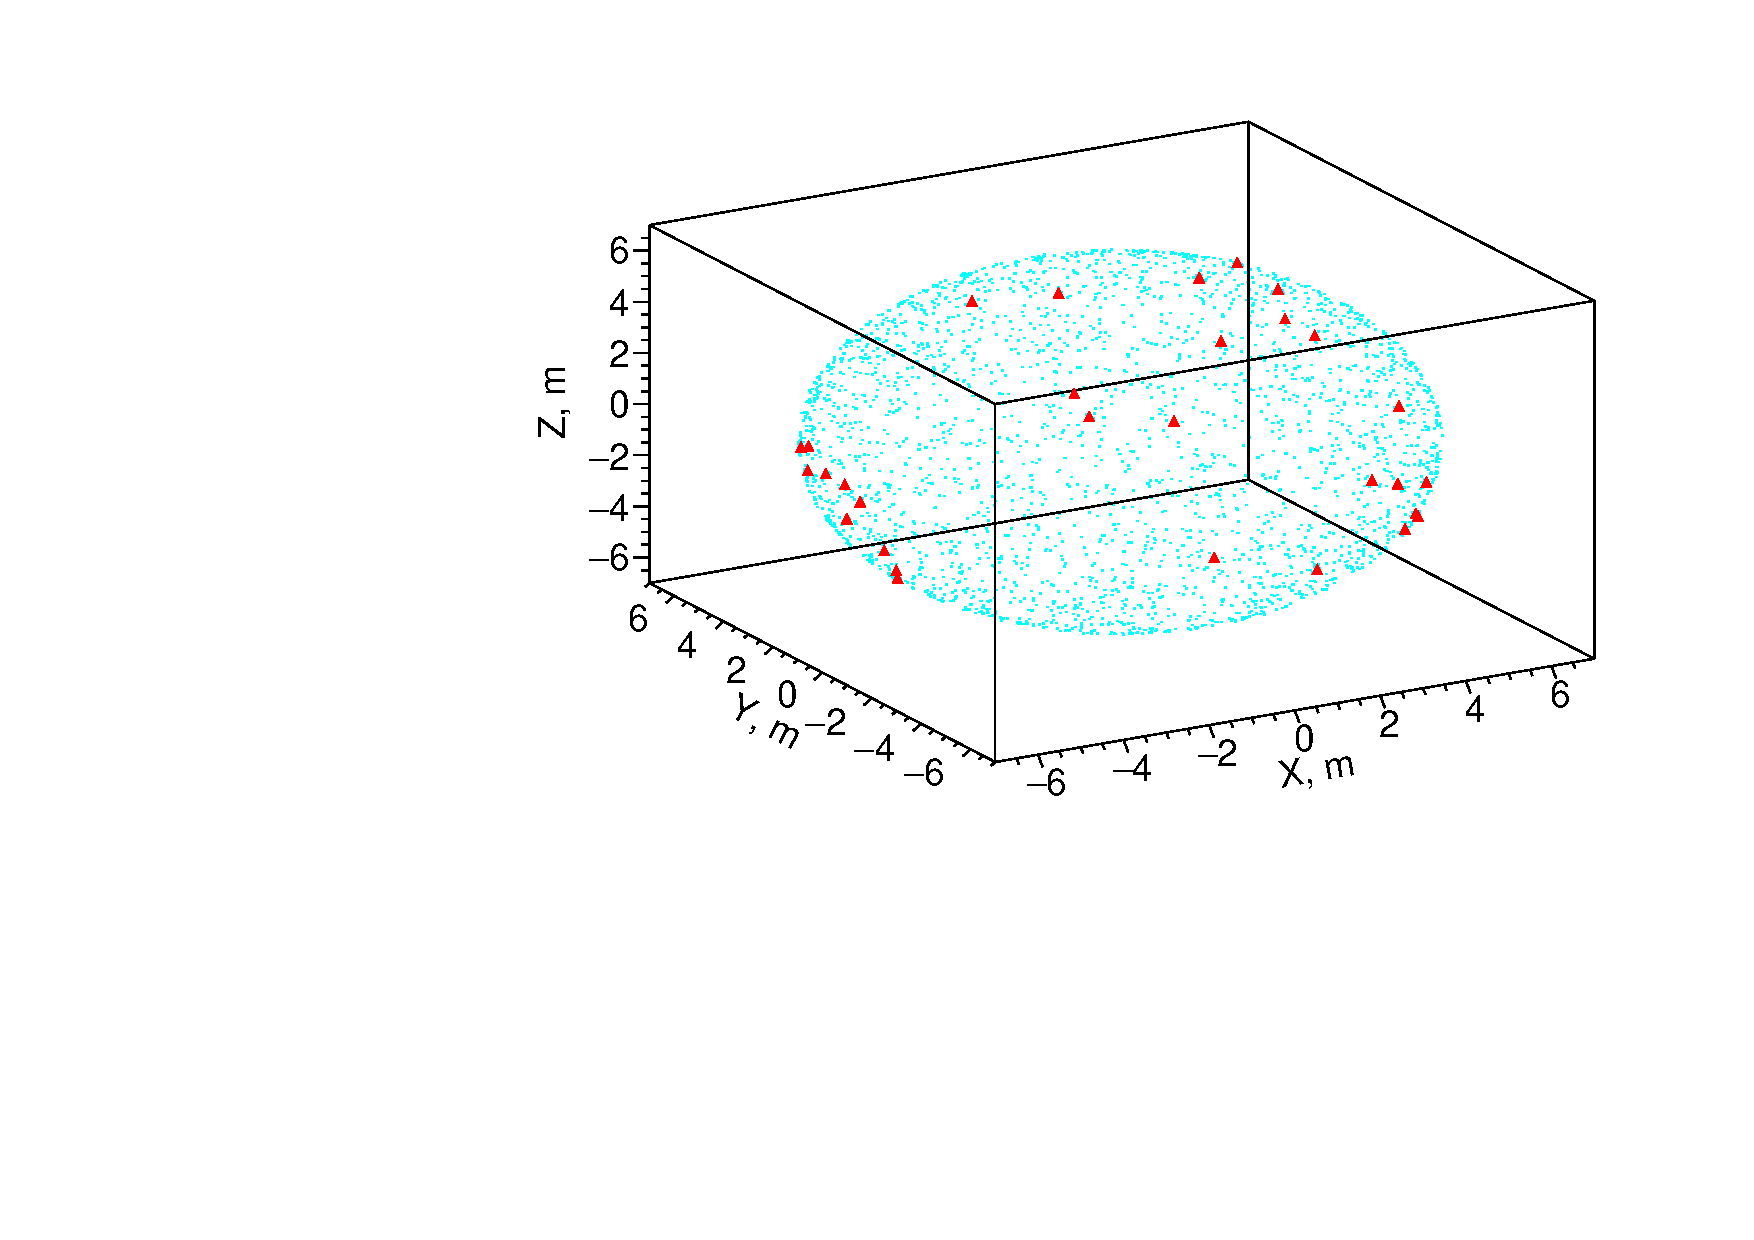
\includegraphics[width=0.3\textwidth]{hDisplay_topology180_2p529MeVTot}
  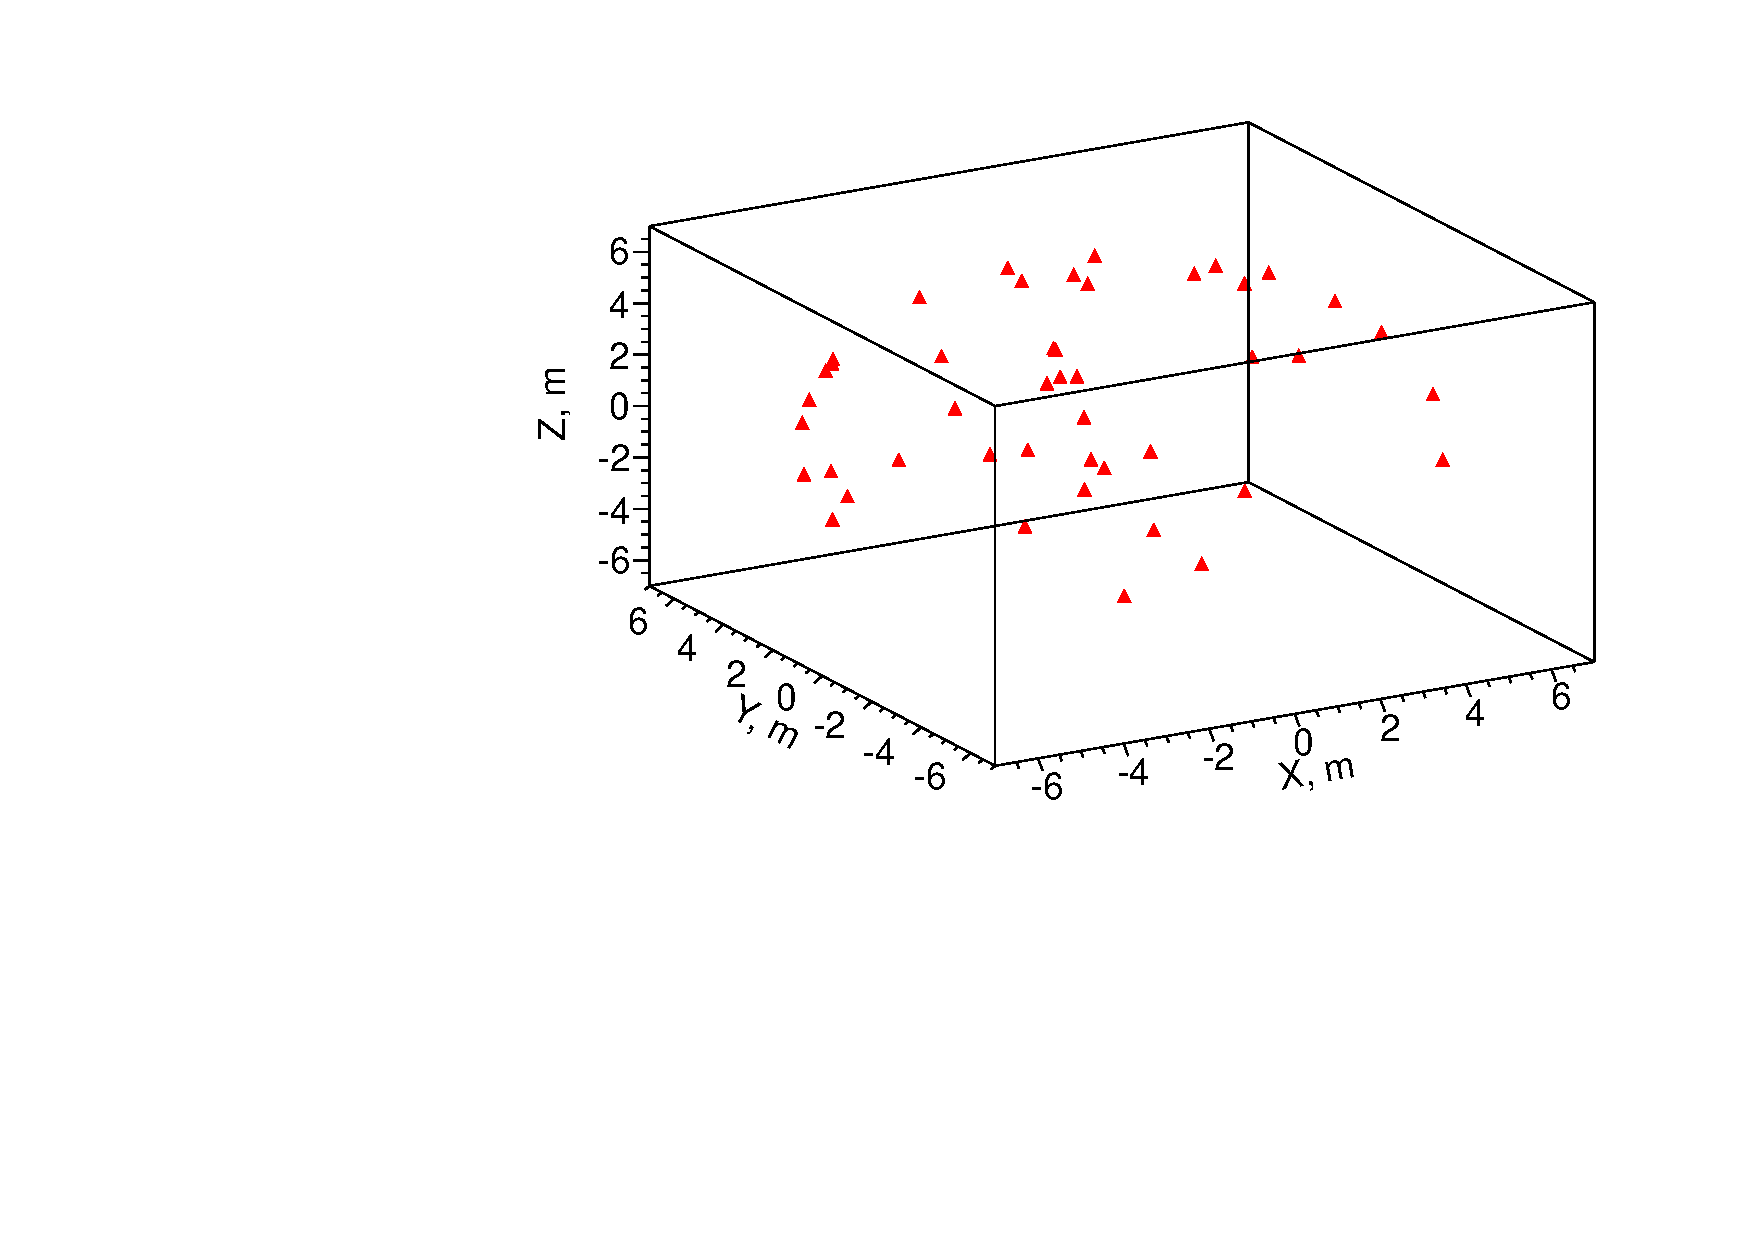
\includegraphics[width=0.3\textwidth]{hDisplay_topology90_2p529MeVTot}
  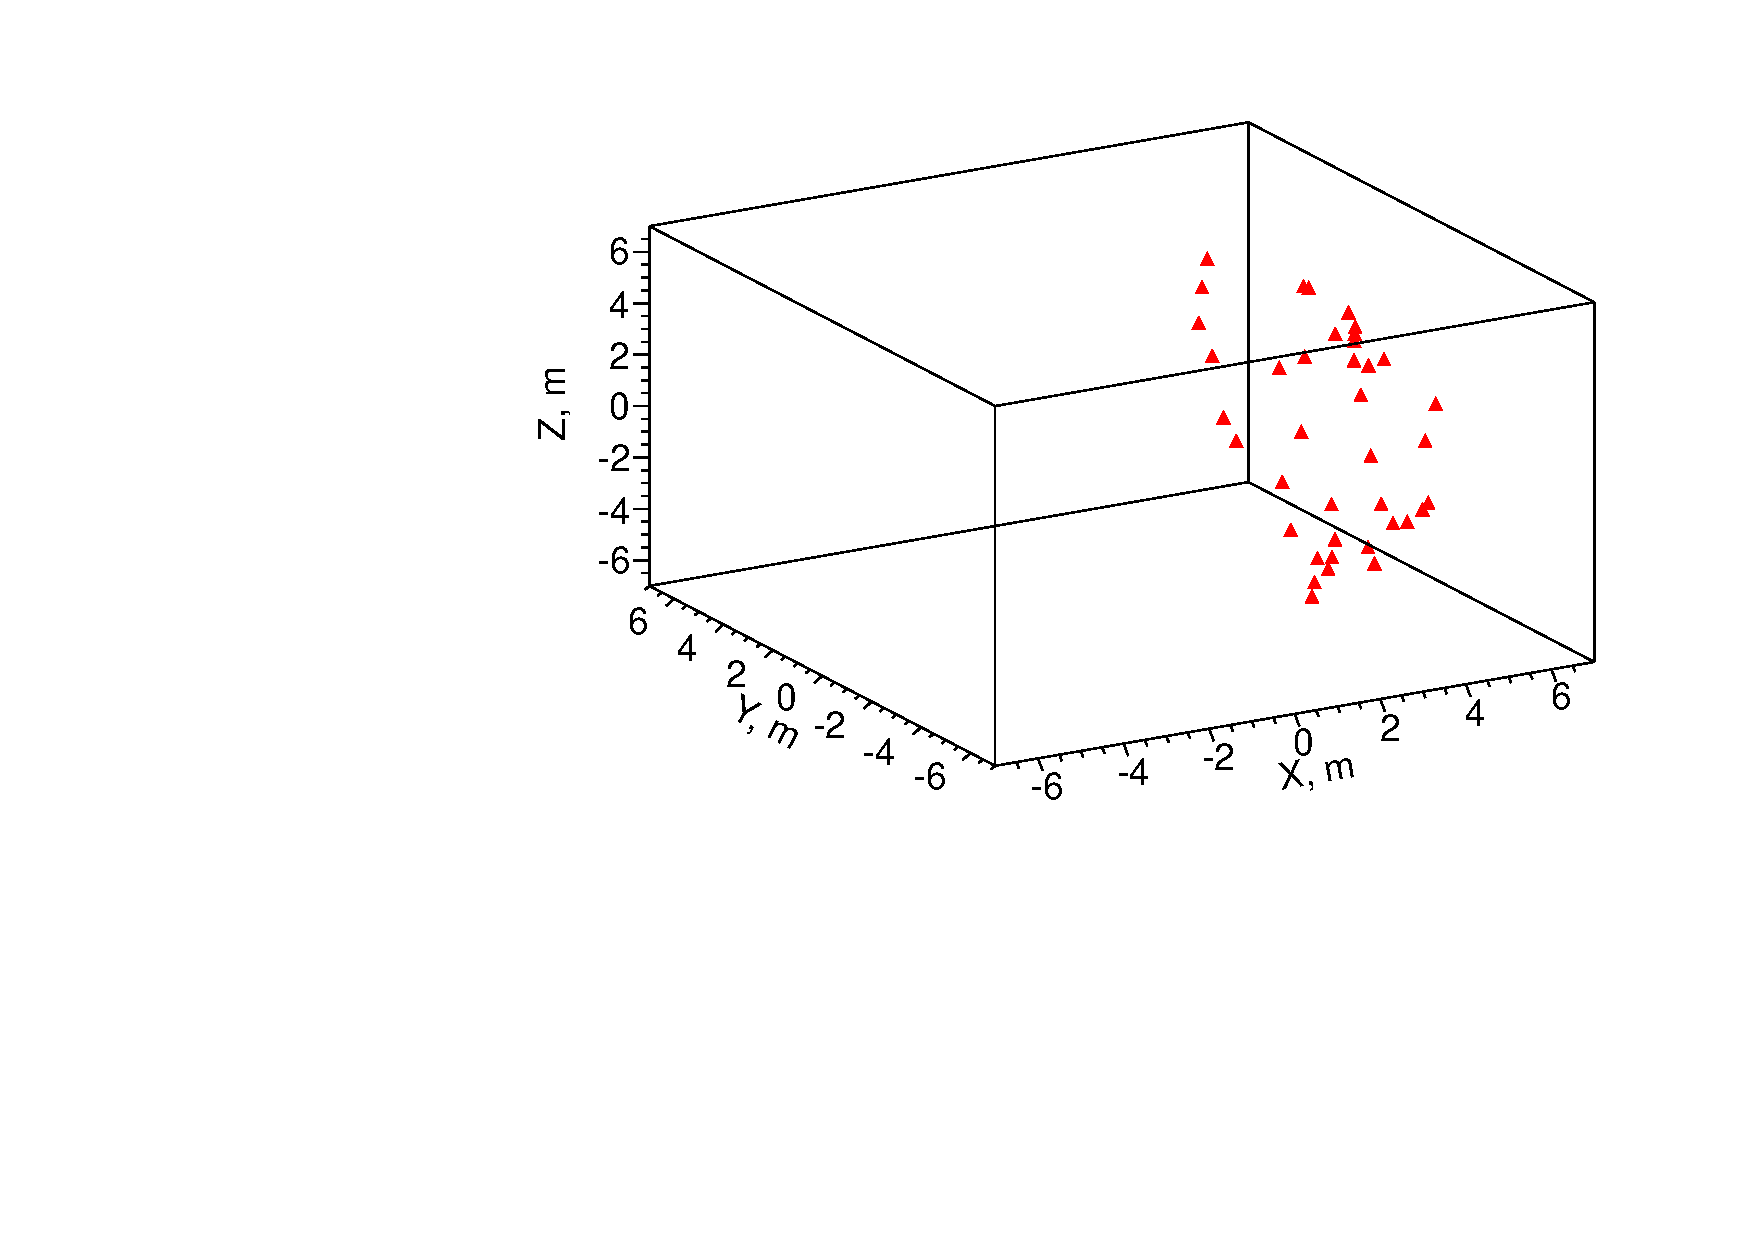
\includegraphics[width=0.3\textwidth]{hDisplay_1el_2p529MeV}
  \end{tabular}
  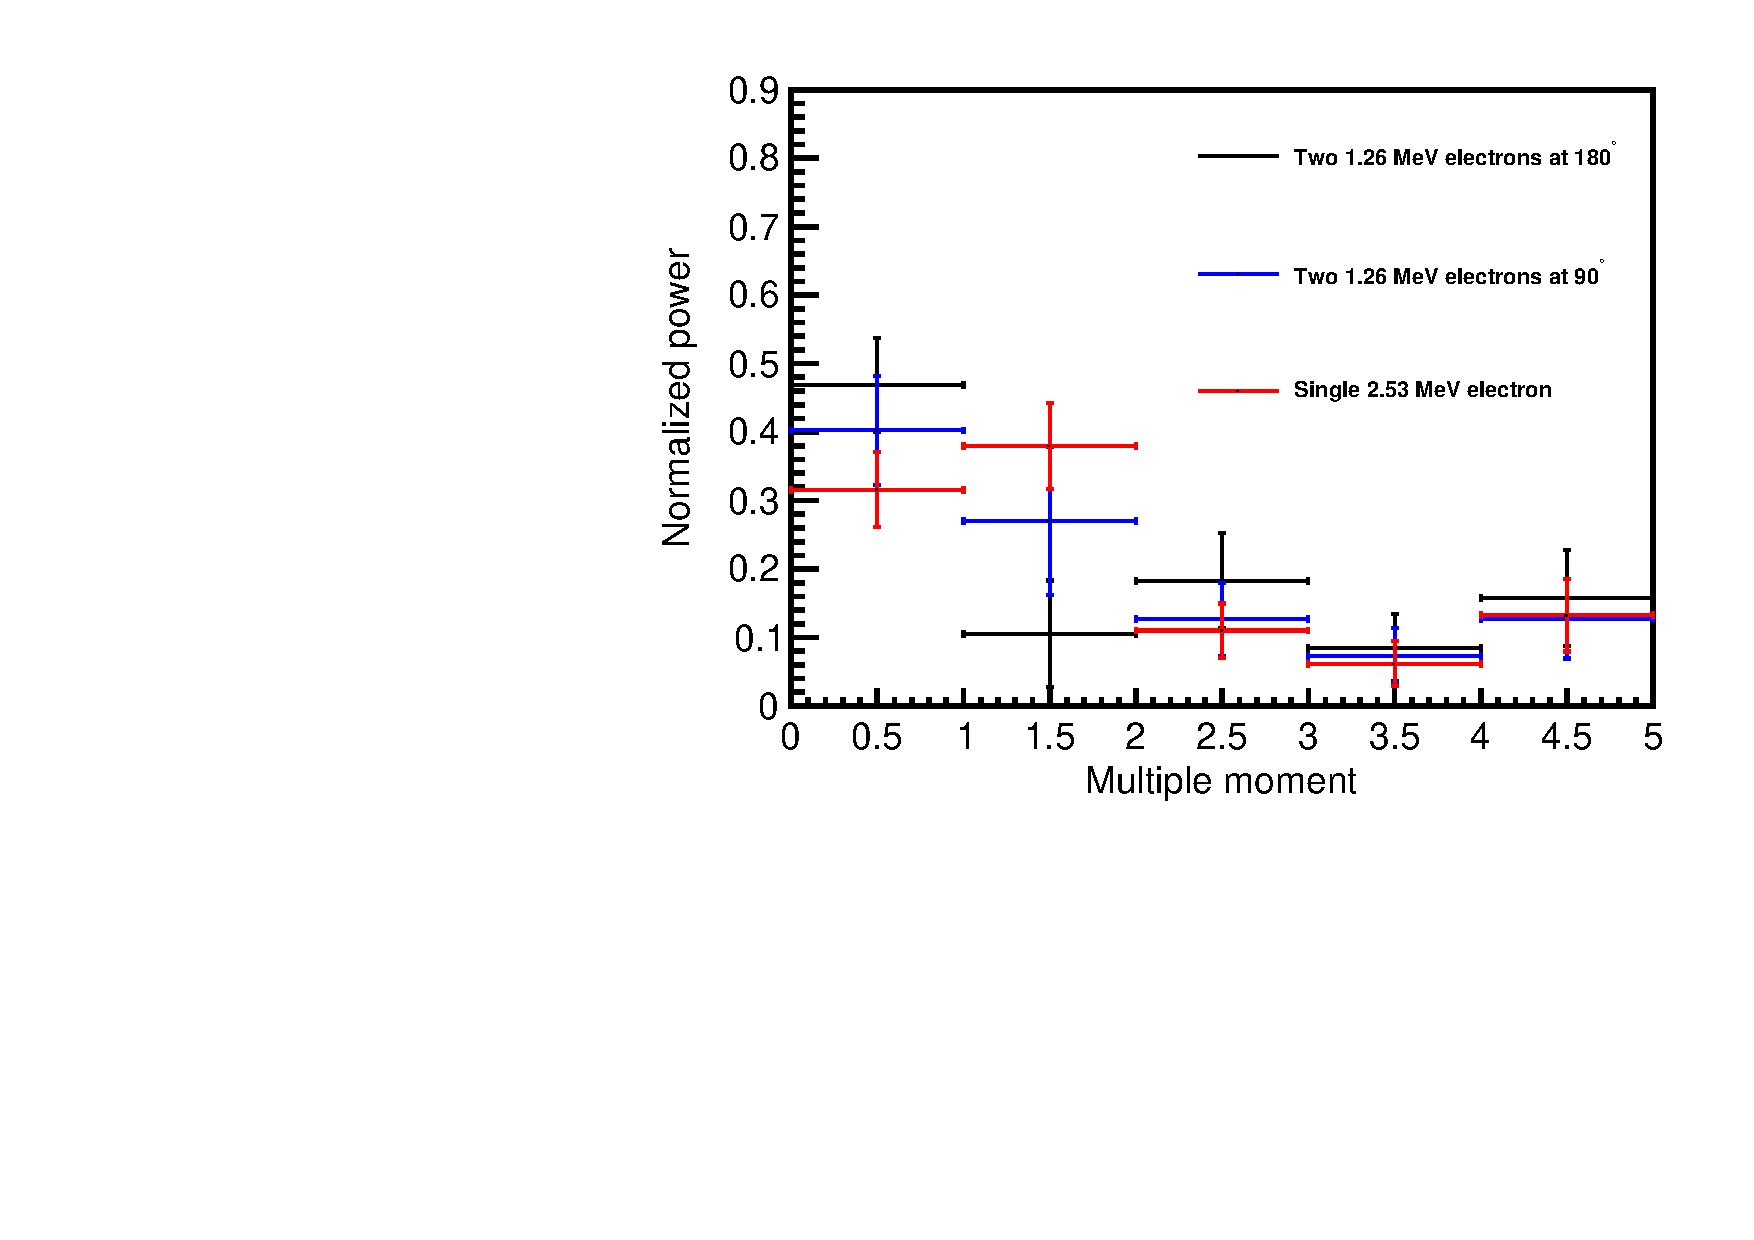
\includegraphics[width=0.9\textwidth]{hMultipleMoment_cheLight_VtxSmear0cm_VtxShiftX0cm_999p9ns_center.pdf}

  \caption{Cherenkov photons distributions on the detector sphere for
    the three representative event topologies: two back-to-back 1.26~MeV
    electrons (\emph{left}), two 1.26~MeV electrons at 90$^{\circ}$
    angle (\emph{middle}), and a single 2.529~MeV electron
    (\emph{center}).  All electrons originate at the center of the
    detector. One randomly selected event is chosen for each
    category. Default QE is applied.}
  \label{fig:Display_top_2p5MeV}
\end{figure*}

More realistic examples of \Te~ 0\nbb~and \B events simulated at the center of the detector are shown in Fig.~\ref{fig:Display_Te130}. Early photoelectrons (PEs), defined as those PEs from Cherenkov and scintillation light within 33.5~ns of the start of the event, are shown. In this example, the default QE is applied.  In this more realistic example, the uniformly distributed scintillation light makes it more difficult to visually distinguish the event topology. Nevertheless, we show that there is still a sufficient difference in the spatial distribution of the early PEs to separate two-track and single-track events using an analysis of spherical harmonics.

\begin{figure*}[h]
  \centering
  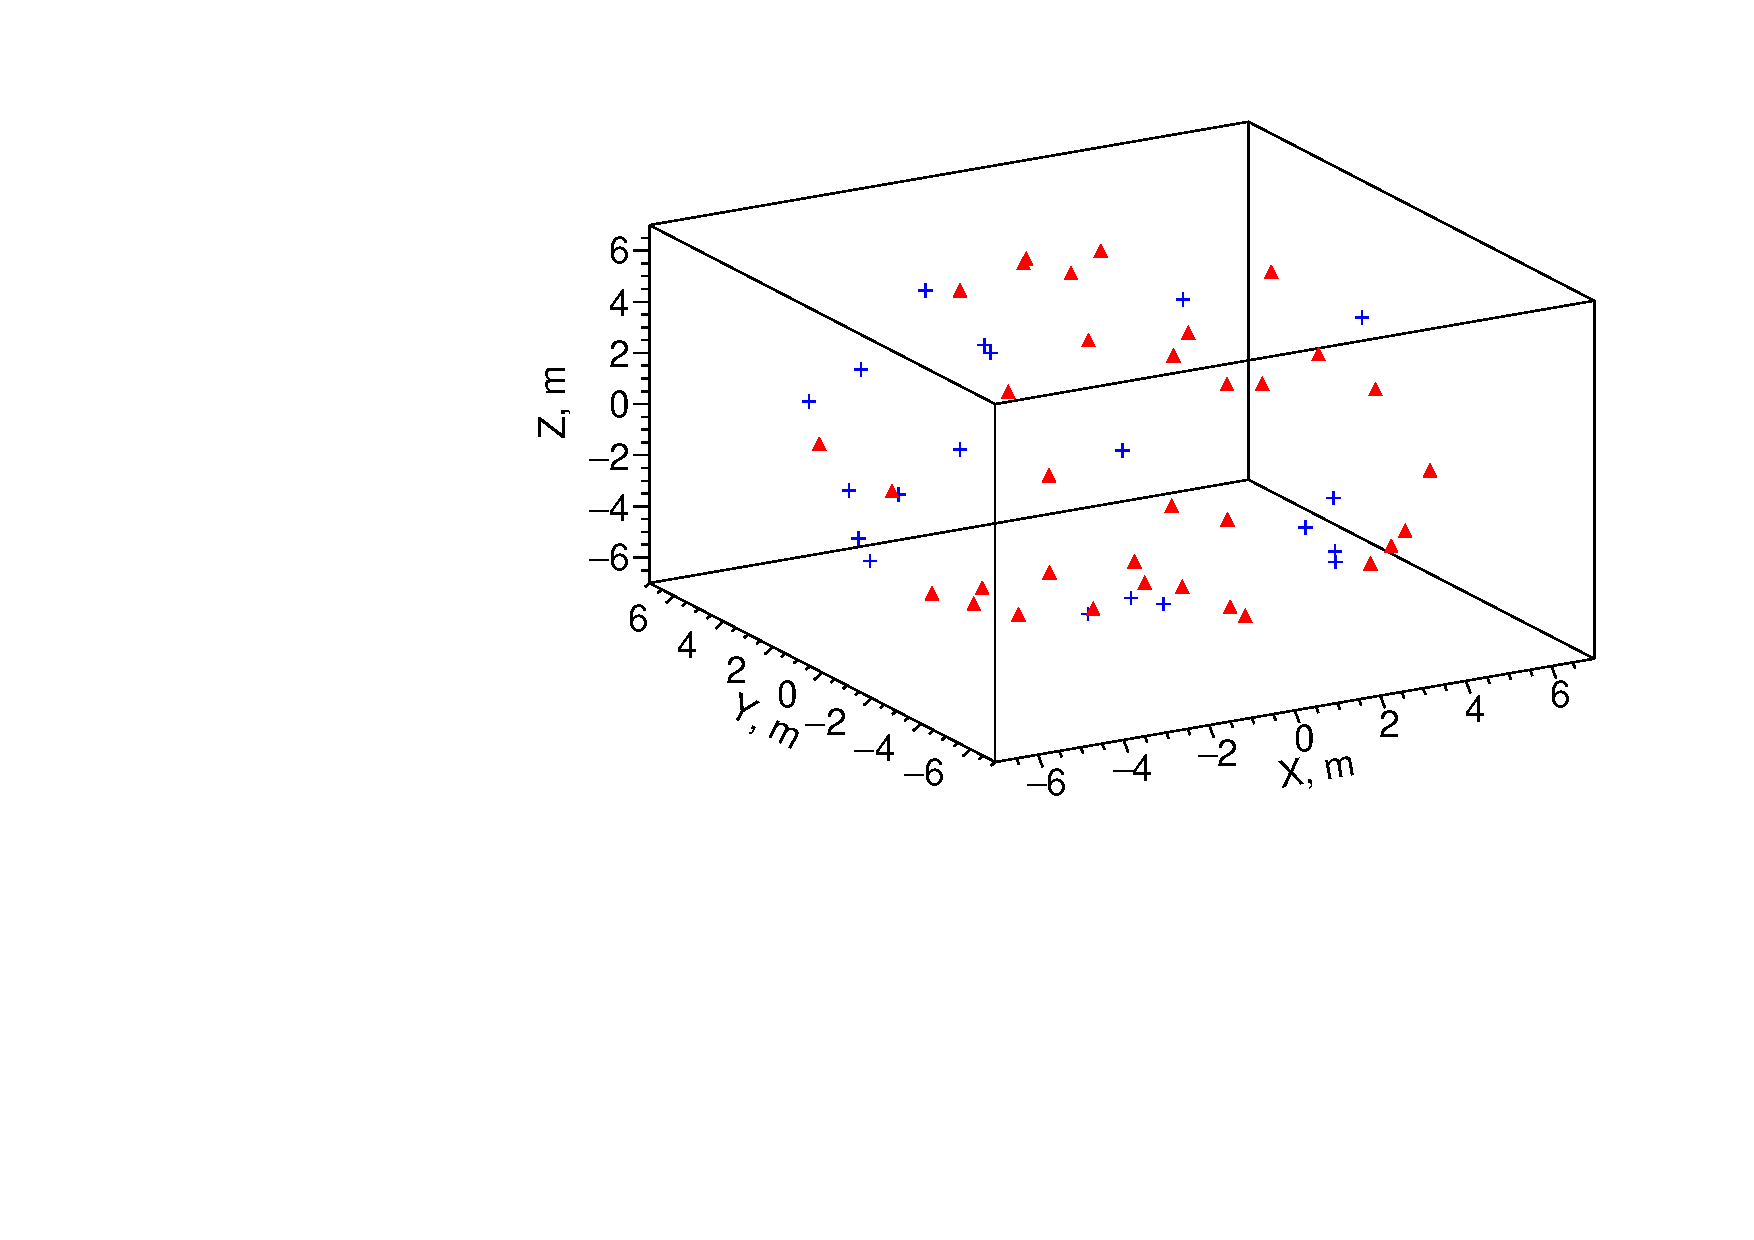
\includegraphics[width=0.45\textwidth]{hDisplay_Te130_evt124_e1257_e1270_cos-0908}
  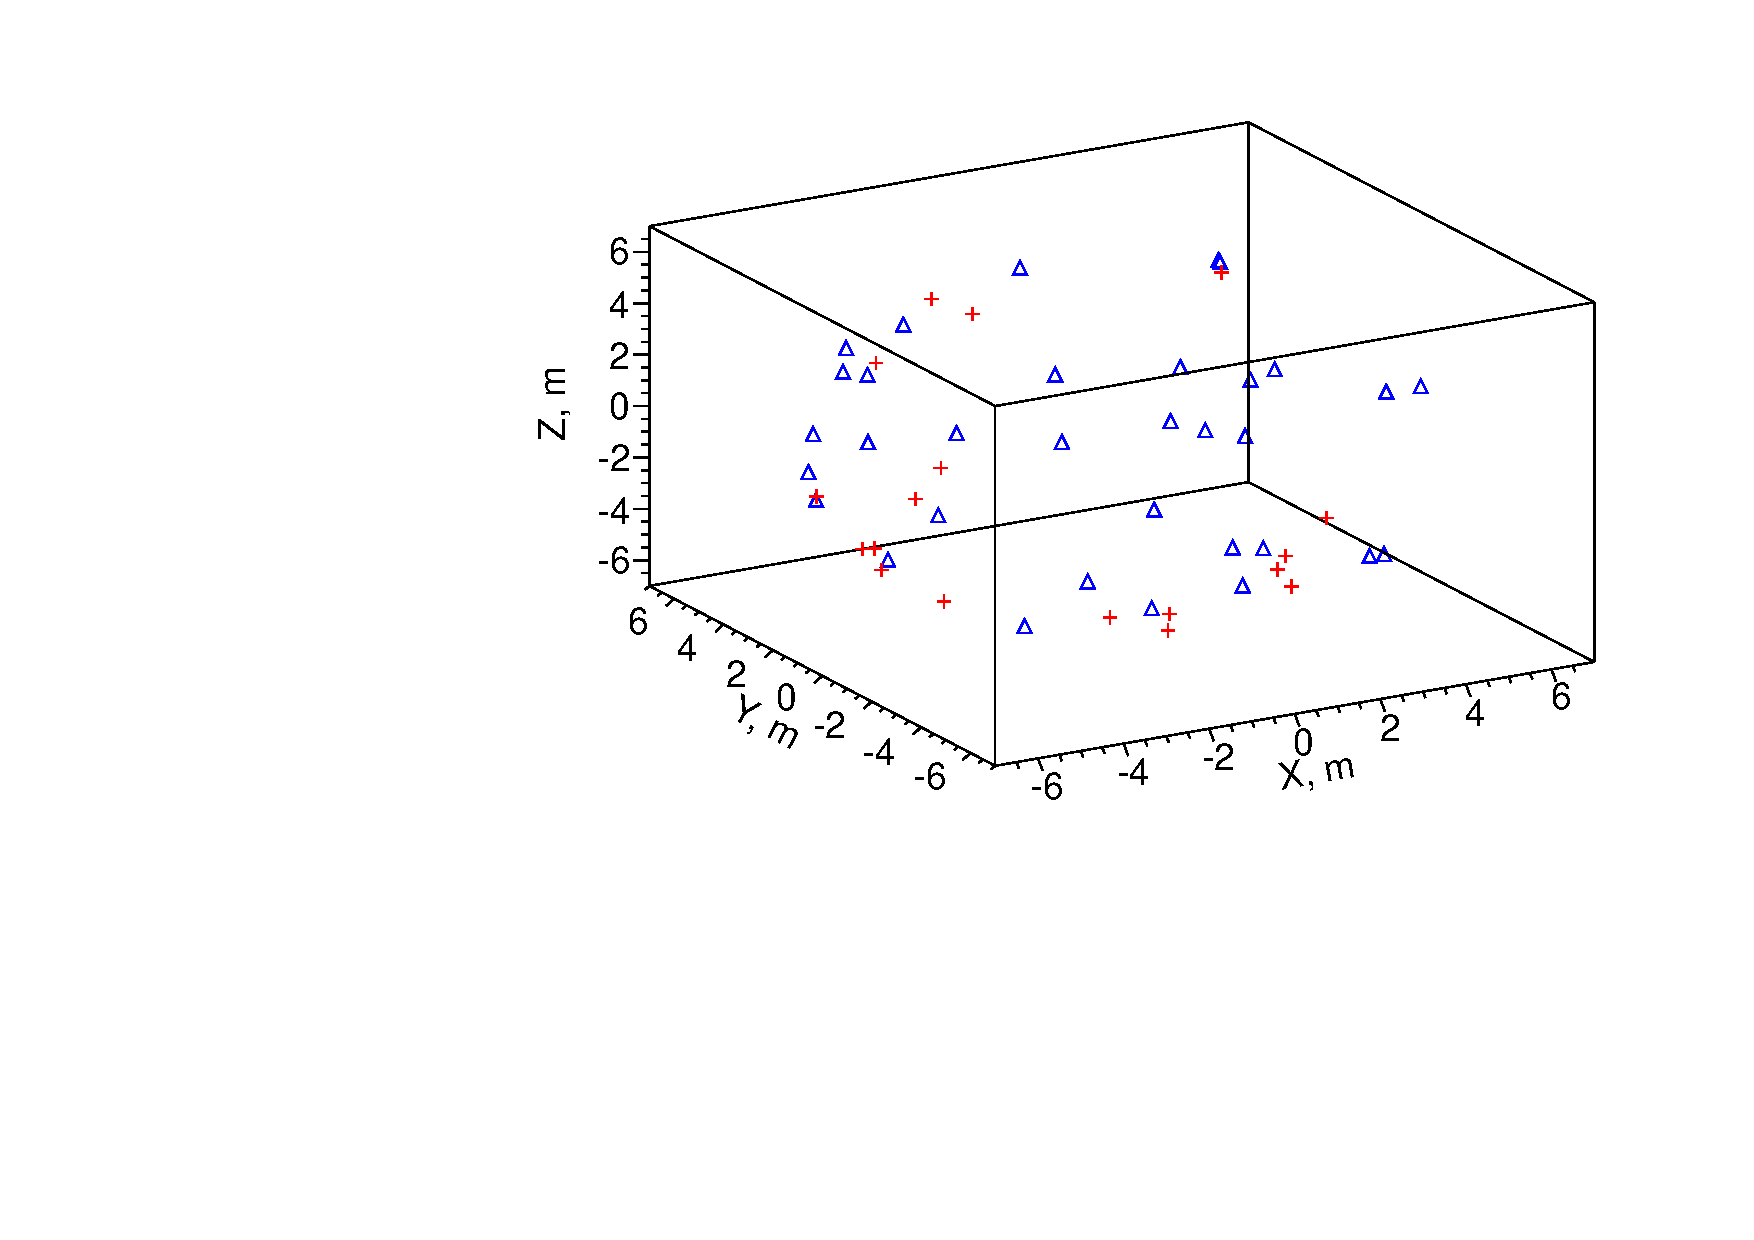
\includegraphics[width=0.45\textwidth]{hDisplay_Te130_evt131_e1264_e1263_cos-0029}
  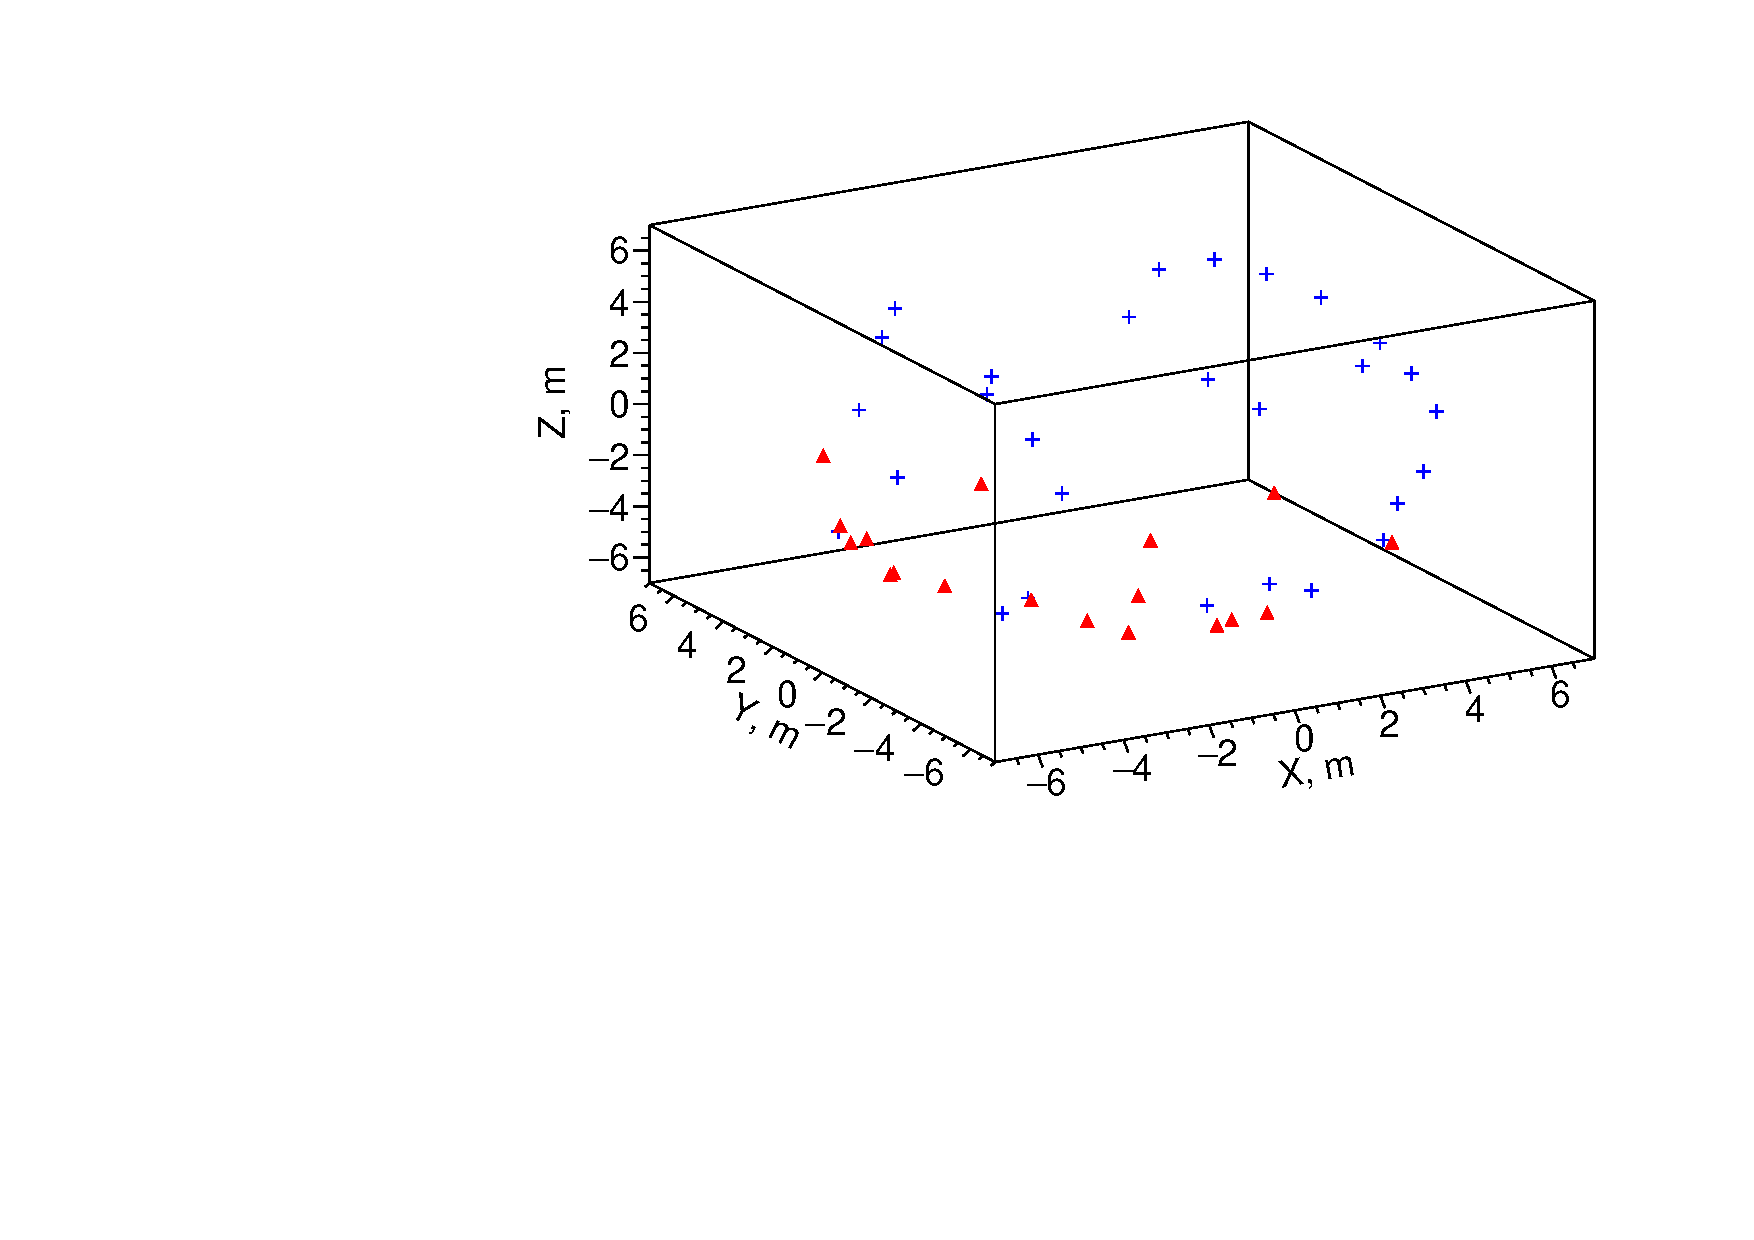
\includegraphics[width=0.45\textwidth]{hDisplay_Te130_evt352_e1186_e1340_cos0888}
  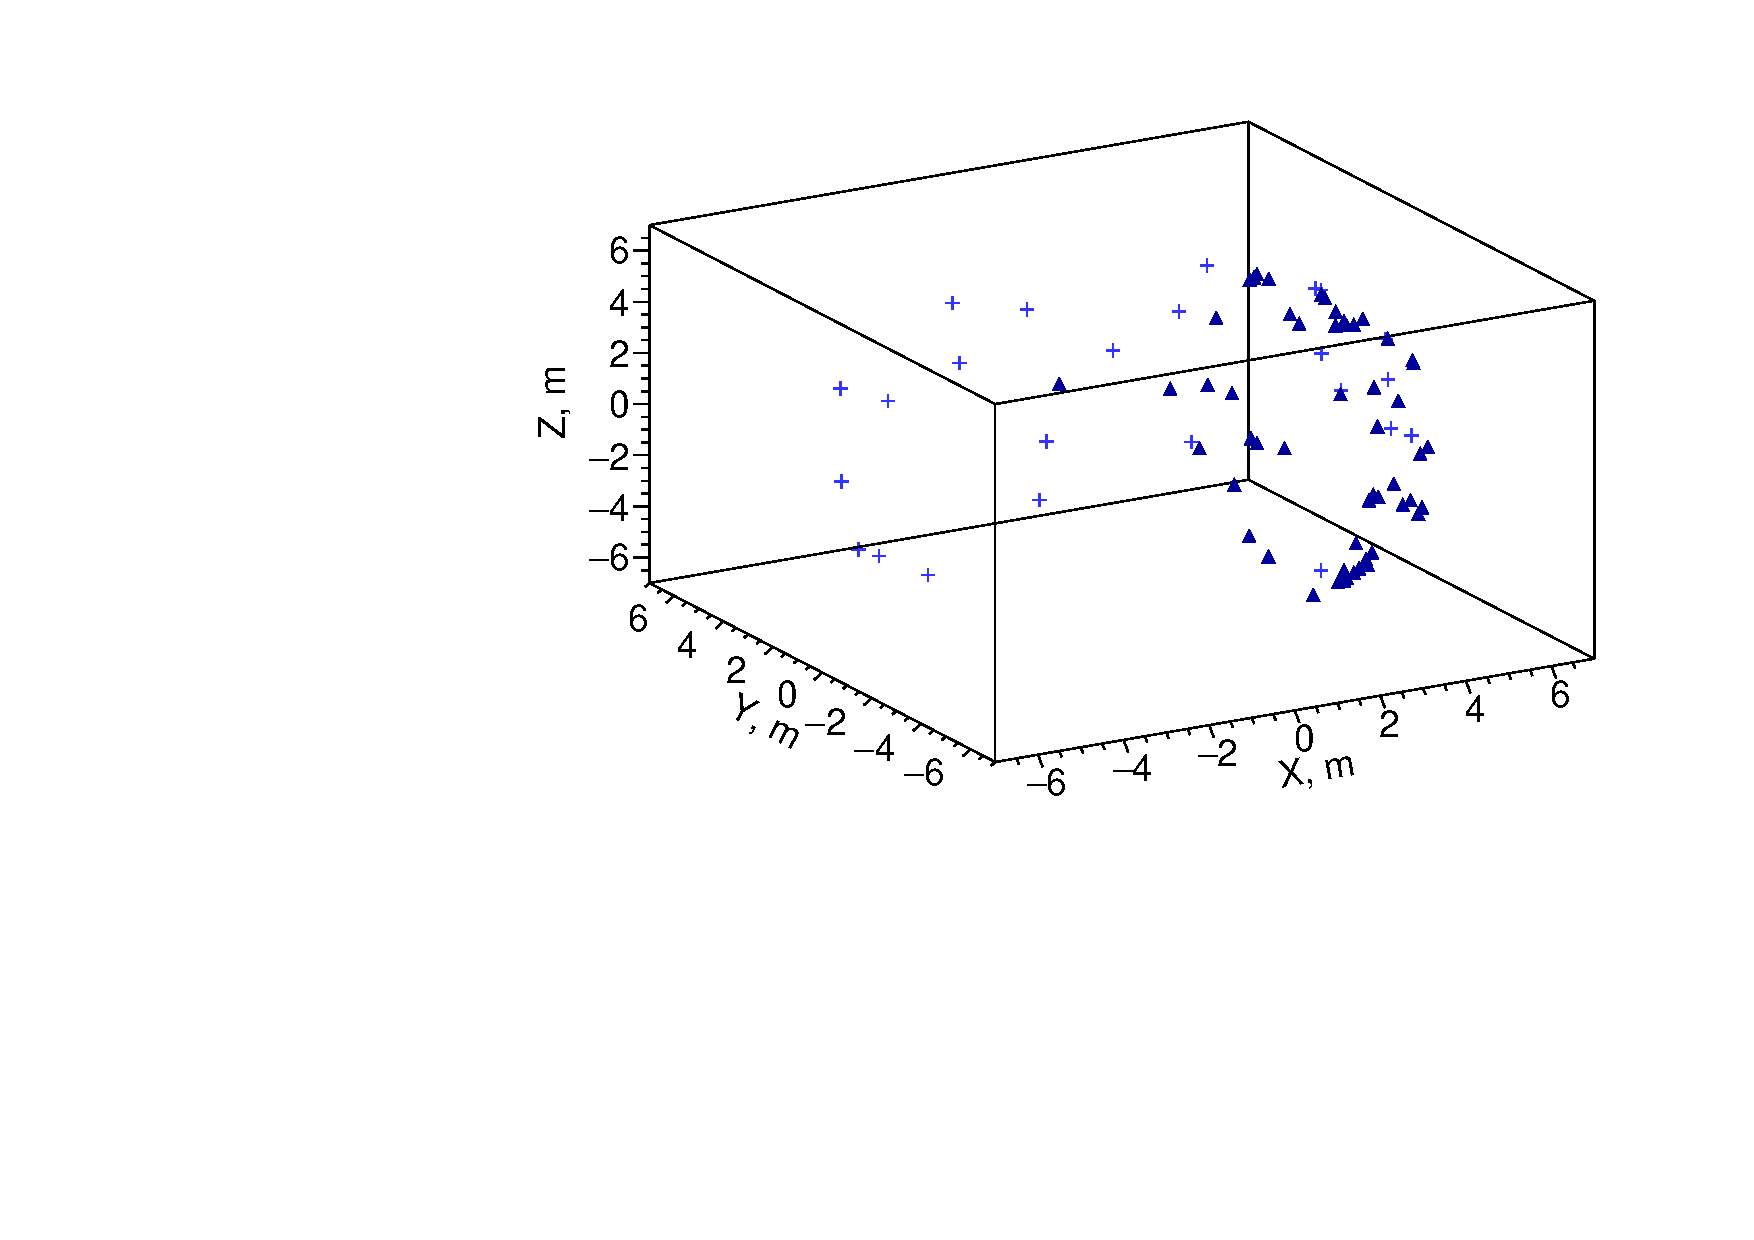
\includegraphics[width=0.45\textwidth]{hDisplay_1el_2p529MeV_33p5ns}
  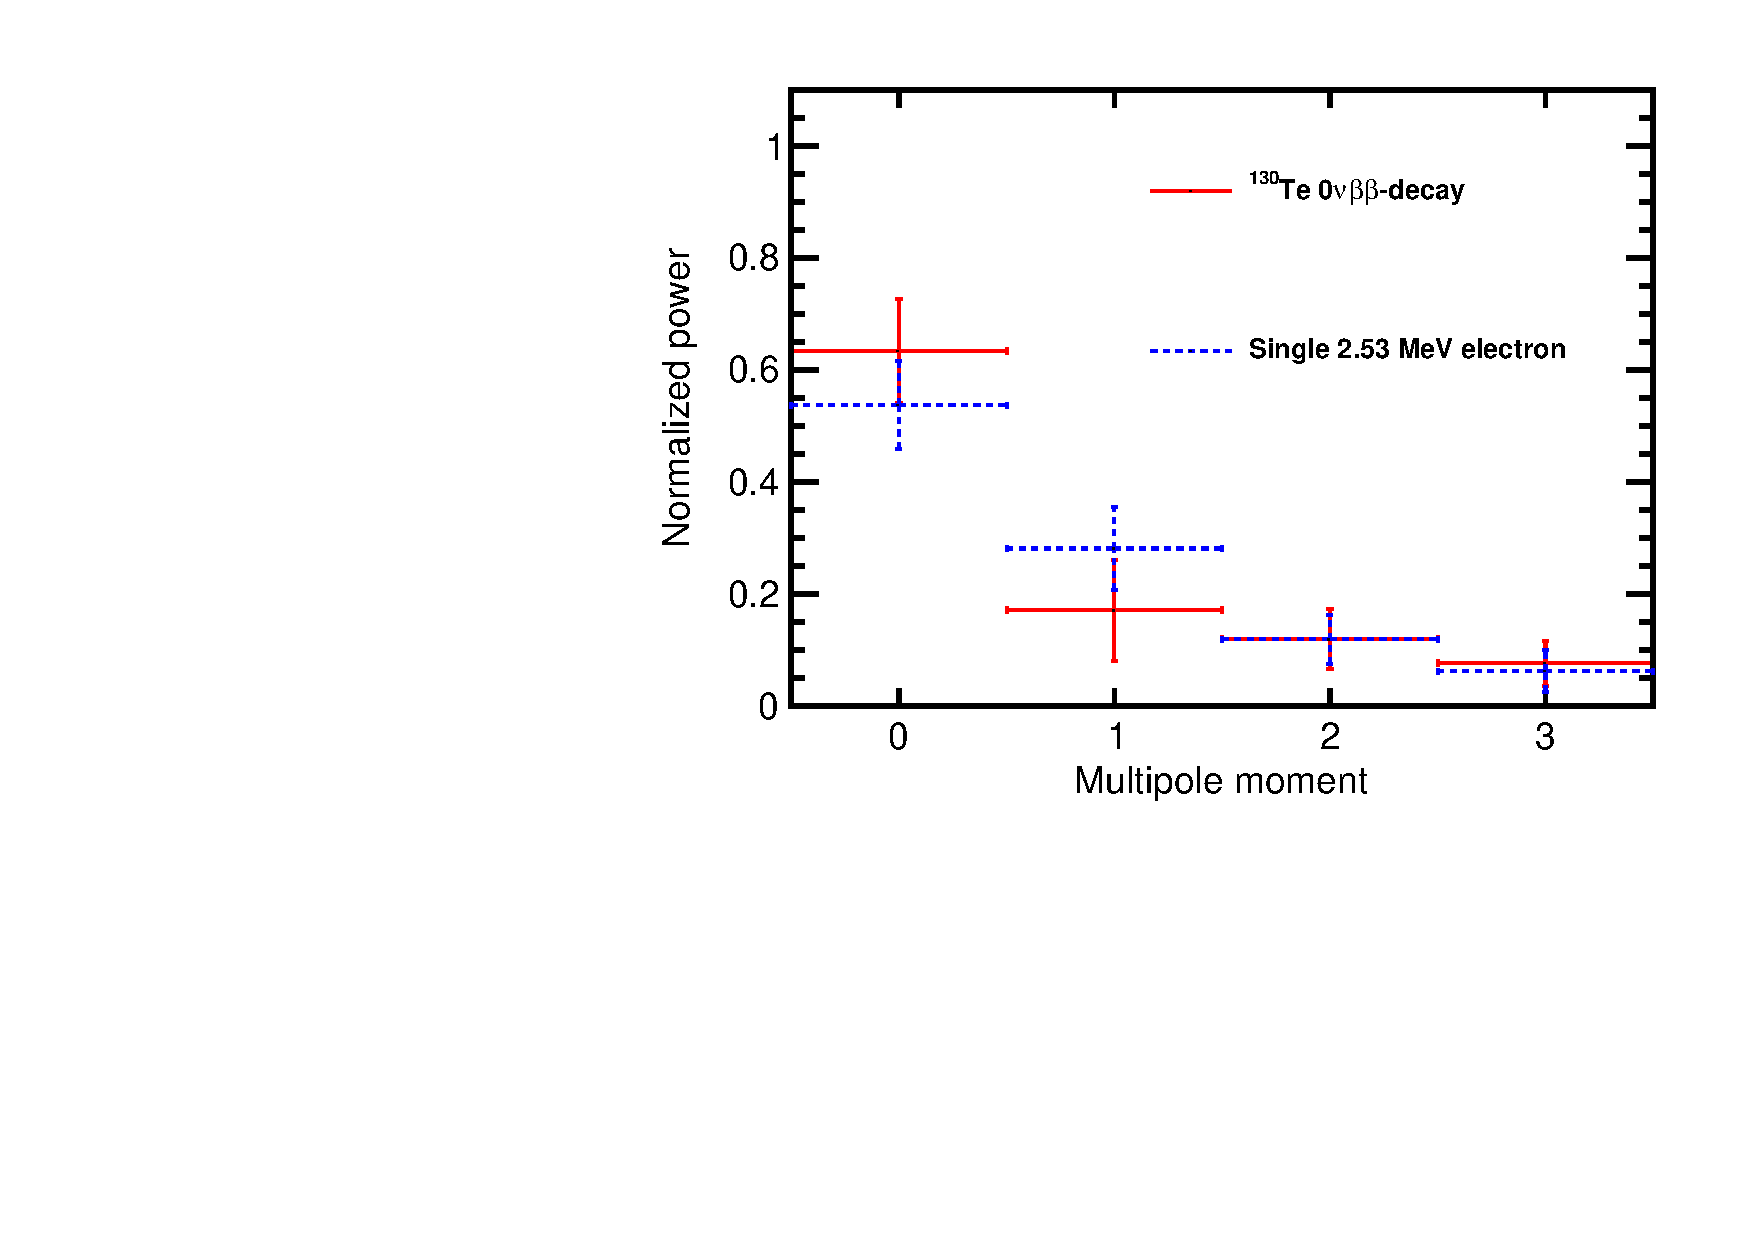
\includegraphics[width=0.9\textwidth]{hMultipleMomentSignal_allLight_VtxSmear0cm_VtxShiftX0cm_33p5ns_center.pdf} 
  \caption{Examples of PEs position on the detector sphere after time
    cut of 33.5ns. PEs from Cherenkov (\emph{red}) and scintillation
    light (\emph{blue}) are compared. \emph{Top left:} $^{130}$Te
    0{\nbb} decay back-to-back electrons: $E_1$=1.257~MeV,
    $E_2$=1.270~MeV, cos($\theta$)=-0.908. \emph{Top right:}
    $^{130}$Te 0{\nbb} decay electrons at $\sim$90$^{\circ}$:
    $E_1$=1.264~MeV, $E_2$=1.263~MeV,
    cos($\theta$)=-0.029. \emph{Bottom left:} $^{130}$Te 0{\nbb} decay
    electrons at $\sim$0$^{\circ}$: $E_1$=1.186~MeV, $E_2$=1.340~MeV,
    cos($\theta$)=0.888. \emph{Bottom right:} 2.529~MeV single
    electron. Events are simulated at the center of the
    detector. Default QE is applied.}
\label{fig:Display_Te130}
\end{figure*}

%% Maybe we should move this discussion to after the analysis is introduced.  
%For a quantitative description of the difference in the event topology, we analyze spherical harmonics of the photon distributions on the detector sphere. We construct rotation invariant variables and compare their value between signal and background events. As shown in the bottom part of Fig.~\ref{fig:Display_Te130}, 0\nbb-decay events become indistinguishable from single track topology when the angle between the two electrons is small (i.e. they form two degenerate tracks). Event topologies of 0\nbb-decay and \B events are also very similar when only one electron from 0\nbb-decay is above the Cherenkov threshold. Therefore spherical harmonics analysis is most efficient for events with large angular separation between the two electrons and when both electrons are above Cherenkov threshold. 
%
%In this paper we focus on topological differences between two-tracks and single-track events and do not make any attempt to use absolute directional information to suppress single track events. For example, one might reject events where the direction of the track is consistent with the direction of solar neutrinos. Once a single track topology is established, one can use a centroid method (see Ref.~\cite{Directionality}) to reconstruct directionality of the track (or two degenerate tracks) in order to suppress events that are aligned with the direction of \B solar neutrinos.

\subsection{Description of Spherical Harmonics Analysis}

The central strategy of the analysis is to construct rotationally invariant variables that can be used to separate signal and background events. To this end, let the  function $f(\theta,\phi)$ represent the PE distribution on the detector surface. The function $f(\theta,\phi)$ can be decomposed into a sum of spherical harmonics:

\begin{eqnarray}
\label{eq1}
f(\theta,\phi) = \sum_{l=0}^{\infty} \sum_{m=-l}^{l} f_{lm} Y_{lm}(\theta,\phi),
\end{eqnarray}

where $Y_{lm}$ are Laplace's spherical harmonics defined in a real-value basis using Legendre polynomials $P_l$:

\begin{eqnarray}
\label{eq2}
Y_{lm} = \left\{
  \begin{array}{@{}ll@{}}
    \sqrt{2}N_{lm}P_l^m(cos\theta)cos~m\phi, & \text{if}\ m>0 \\
    N_{lm} = \sqrt{\frac{(2l+1)}{4\pi} \frac{(l-m)!}{(l+m)!}}, & \text{if}\ m=0 \\
    \sqrt{2}N_{l|m|}P_l^|m|(cos\theta)sin~|m|\phi, & \text{if}\ m<0
  \end{array}\right.
\end{eqnarray}

where the coefficients $f_{lm}$ are defined as
 
\begin{eqnarray}
\label{eq3}
f_{lm} = \int_{0}^{2\pi} d\phi \int_0^{\pi} d\theta sin\theta f(\theta,\phi) Y_{lm}(\theta,\phi).
\end{eqnarray}

Equation~\ref{eq4} defines the power spectrum of $f(\theta,\phi)$ in the spherical harmonics representation, $s_l$, where $l$ is a multiple moment. The power spectrum, $s_l$, is invariant under rotation. It is unique to each of the functions $f_i(\theta,\phi)$, $i=$1,2,3..., which can not be transformed into each other by rotation.

\begin{eqnarray}
\label{eq4}
s_l = \sum_{m=-l}^{m=l} |f_{lm}|^2
\end{eqnarray}

%% here
%One can consider PEs distribution for each of 0\nbb-decay signal or background event as a function $f_i(\theta,\phi)$. Events with similar power spectrum would correspond to PE distributions on the detector sphere that can be closely aligned by a rotation. Such PE distributions belong to events with similar topology.

The topology of 0\nbb~signal or background in a spherical detector determines the distribution of the PE's on the detector sphere, and, therefore, a set of $s_l$'s. These values can serve as a quantitative figure of merit for different event topologies. The rotation invariance of $s_l$'s ensures that this figure of merit does not depend on the orientation of the event with respect to the chosen coordinate frame.

Sum of $s_l$'s over all multiple moments equals to the L2 norm of the function $f(\theta,\phi)$:

\begin{eqnarray}
\label{eq5}
\sum_{l=0}^{\infty} s_l = \int_{\Omega} |f(\theta,\phi)|^2 d\Omega.
\end{eqnarray}

Therefore, the normalized power spectrum,

\begin{eqnarray}
\label{eq6}
S_l = \frac{s_l}{\sum_{l=0}^{\infty} s_l} =  \frac{s_l}{\int_{\Omega} |f(\theta,\phi)|^2 d\Omega},
\end{eqnarray}

can be used to compare shapes of various functions $f(\theta,\phi)$ with different normalization. The total number of PEs detected on the detector sphere fluctuates from event to event, therefore, in all of the following we use the normalized power $S_l$.

Figure~\ref{fig:Moments} compares the normalized power spectra for the three representative event topologies that were previously shown in Fig.~\ref{fig:Display_top_5MeV}. We note that most of the information is contained in the power spectrum with $l<$6. In most cases we found that there is no need to calculate $S_l$ for $l>$3 to achieve maximal separation between 0\nbb~and \B~events. This limit is due to fluctuations in the PE distribution that produce a lot of noise in the power spectrum for higher orders of multiple moments.

\begin{figure*}[h]
  \centering
  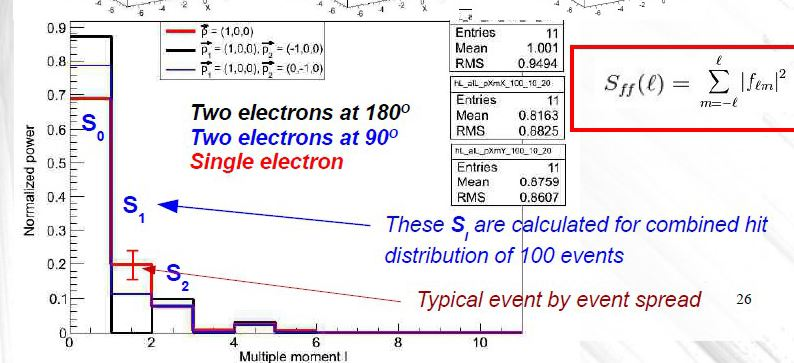
\includegraphics[width=0.95\textwidth]{Multiple_moment.JPG}
  \caption{Average $S_l$ values for two electrons at 180 degree
    (\emph{color1}) and 90 degree (\emph{color2}) 1.5~MeV each and a
    single electron (\emph{color3}) with the energy of 3~MeV. Error
    bars are RMS values of each corresponding individual $S_l$
    distribution (each consists of 1000 events simulated at the center
    of the detector) indicating typical event-by-event variation.}
\label{fig:Moments}
\end{figure*}

%For a quantitative description of the difference in the event topology, we analyze spherical harmonics of the photon distributions on the detector sphere. We construct rotation invariant variables and compare their value between signal and background events. 

As shown in the bottom part of Fig.~\ref{fig:Display_Te130}, 0\nbb~events become indistinguishable from single-track events when the angle between the two electrons is small (i.e. they form two overlapping tracks). Event topologies of 0\nbb~and \B~events are also very similar when only one electron from 0\nbb~ is above the Cherenkov threshold. Therefore spherical harmonics analysis is most efficient for events with large angular separation between the two electrons and when both electrons are above Cherenkov threshold. 

Being able to distinguish between two-tracks and single-track events using the spherical analyses can allow further cuts to be made.  For example, one might use absolute directional information to suppress single track events where the direction of the track is consistent with the location of a known background such as the sun. Once a single track topology is established, one can use a centroid method (see Ref.~\cite{Directionality}) to reconstruct directionality of the track (or two degenerate tracks) in order to suppress events that are aligned with the direction of \B~solar neutrinos.

\subsection{Spherical Harmonics Analysis and Off-center Events}

The calculation of the normalized power spectrum, $S_I$, above, assumes that the coordinate system is located at the location of the interaction.  Therefore, in order to compare spherical harmonics for events with vertices not at the center of the detector volume, a coordinate transformation for each photon hit is needed. The necessary transformation applied for each PE within an event is illustrated in Fig.~\ref{fig:SphH_transform}. The solid circle in the Figure has a radius, R, and shows the actual detector boundaries. The dotted circle shows a new sphere with the same radius R, which now has the event vertex in its center. The radius vector of each PE is stretched or shorten to its intersection with this new sphere using the transformation, $\vec{r}^{,}_{PE} = \frac{\vec{a}}{|\vec{a}|} \cdot R$, where $\vec{r}^{,}_{PE}$ is a new radius vector of a PE and $\vec{a}=\vec{r}_{PE} - \vec{r}_{vtx}$ with $\vec{r}_{PE}$ and $\vec{r}_{vtx}$ being radius vectors of the PE and the vertex in the original coordinates, respectively.

\begin{figure*}[h]
  \centering
%  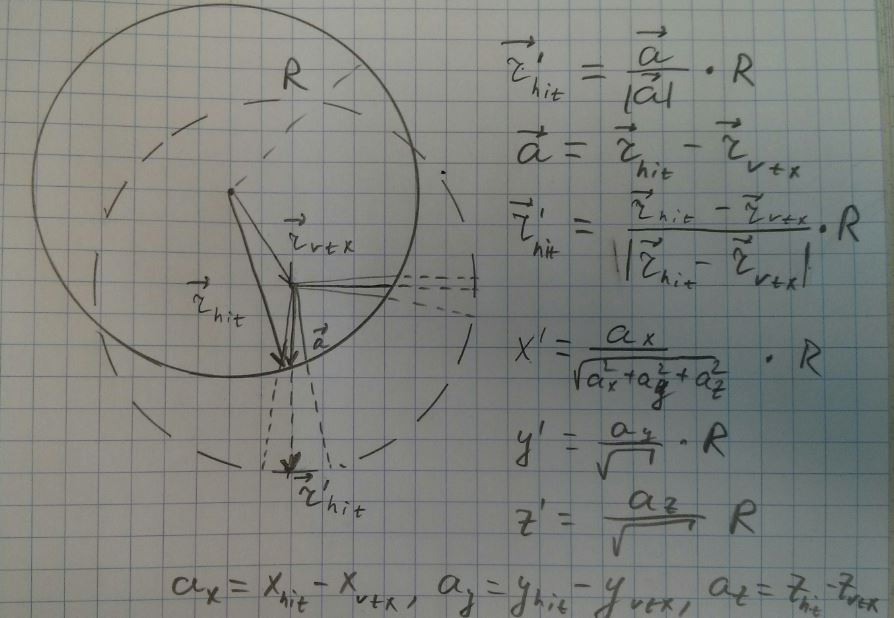
\includegraphics[width=0.95\textwidth]{SphH_transform_sketch.JPG}
  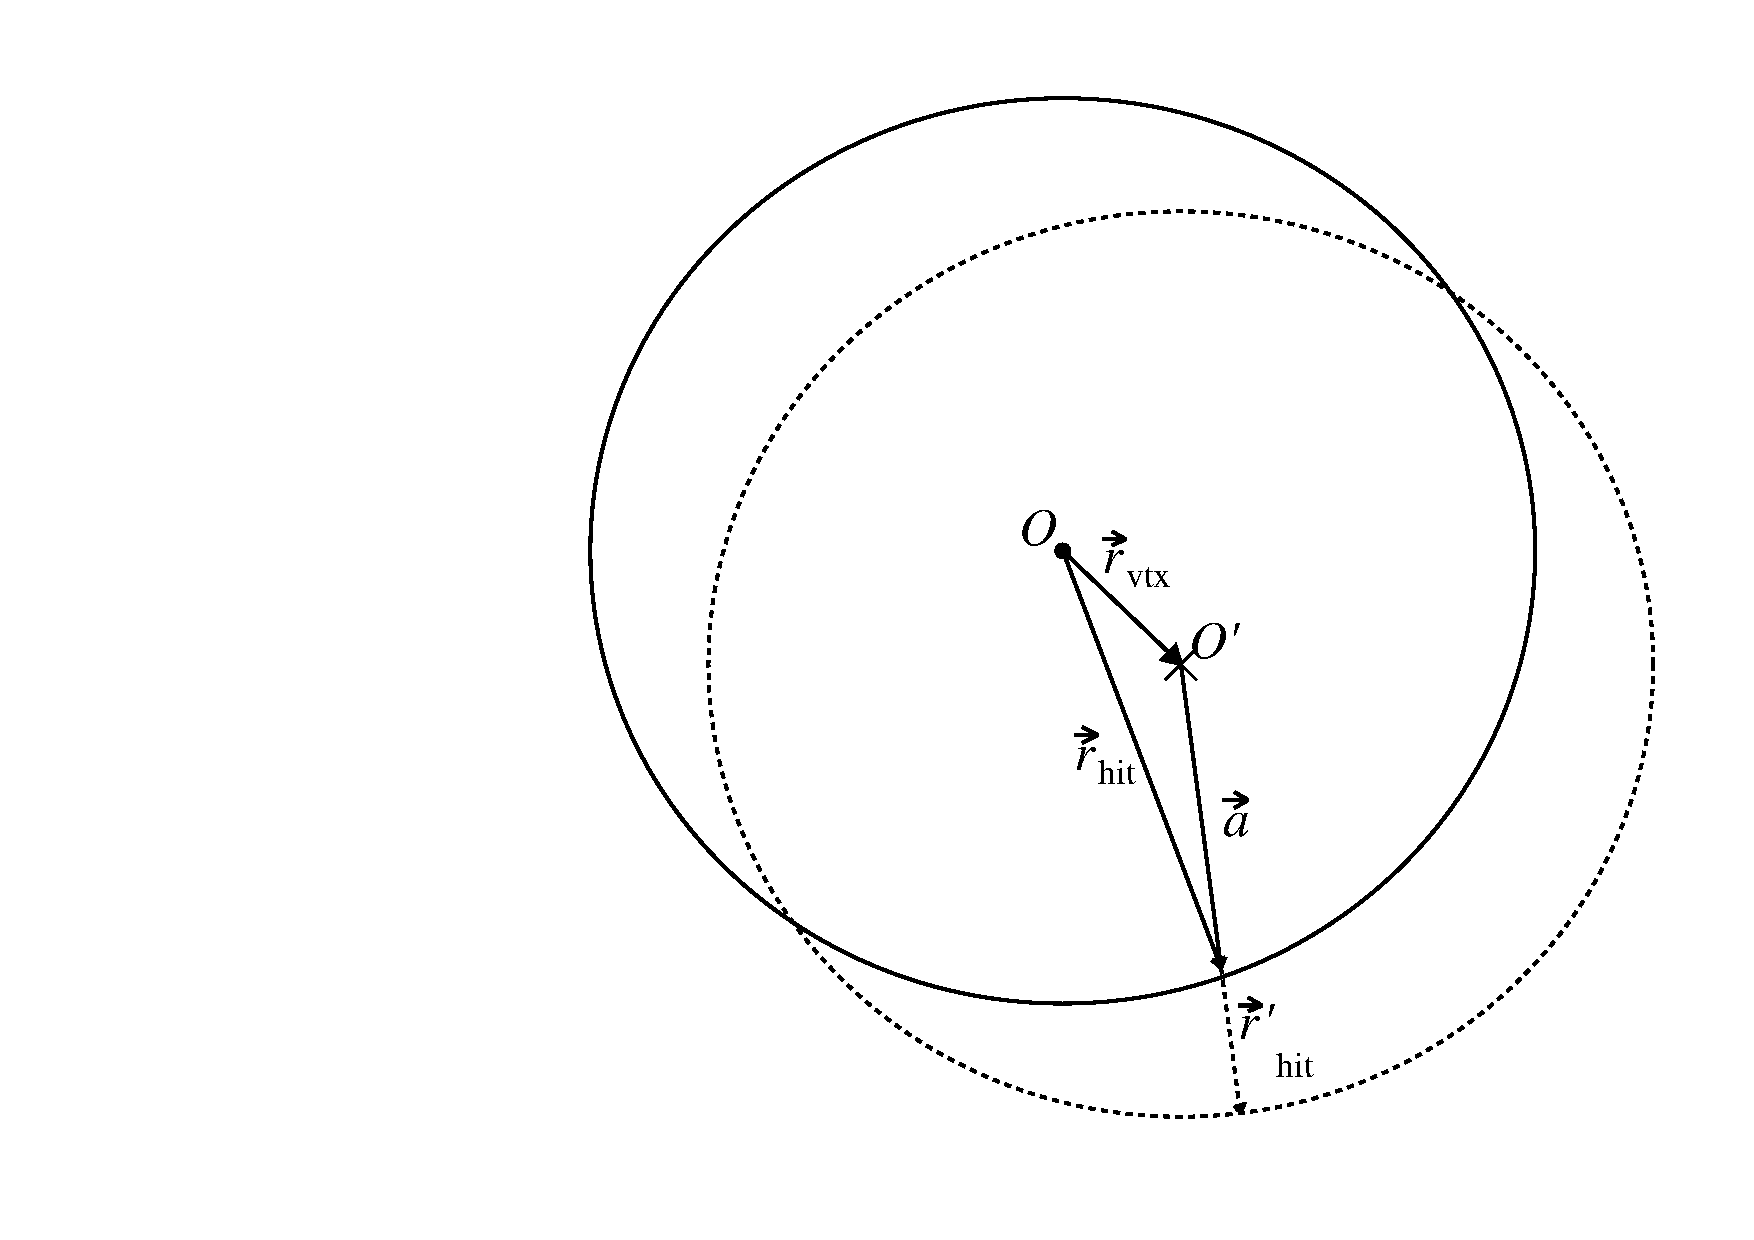
\includegraphics[width=0.95\textwidth]{SphH_transform.pdf}
  \caption{Coordinate transformation applied to events that are
    off-center. Solid circle schematically shows actual detector
    boundaries. Dotted circle shows a new sphere of radius R$=$6.5~m
    with the event vertex position in the center. The radius vector of
    each photon hit is stretched or shorten until intersection with
    this new sphere using transformation $\vec{r}^{,}_{hit} =
    \frac{\vec{a}}{|\vec{a}|} \cdot R$. Where $\vec{r}^{,}_{hit}$ is a
    new radius vector of the photon hit, $R$ is detector sphere radius,
    and $\vec{a}=\vec{r}_{hit} - \vec{r}_{vtx}$ with $\vec{r}_{hit}$
    and $\vec{r}_{vtx}$ being radius vectors of the photon hit and
    vertex position in original coordinates and correspondingly.}
  \label{fig:SphH_transform}
\end{figure*}


\subsection{Implementation of the spherical harmonics analysis}

For each event, we create a 2-D histogram, $\theta$ vs $\phi$, with the distribution of PEs on the detector surface. We then treat this histogram as a function $f(\theta,\phi)$ where the value of the function for any pair of $\theta$ and $\phi$ is equal to the number of PE in the histogram bin corresponding to that pair.

Coefficients $f_{lm}$ from Eq.~\ref{eq3} are calculated using a Monte Carlo integration technique. Variables $S_0$, $S_1$, $S_2$, and $S_3$ are calculated using Eqs.\ref{eq4} - \ref{eq6}.

To illustrate spherical harmonics analysis technique we compare distributions of $S_0$, $S_1$, $S_2$, and $S_3$ for the three representative event topologies described in Sec.~\ref{subsec:topology}. Almost all the information about event topology is carried by Cherenkov light. Therefore we first show spherical harmonics for back-to-back,  90$^{\circ}$ and single track topologies based on Cherenkov PEs only (see Fig.~\ref{fig:SL_topologies_CHE}).

Two top panels of Fig.~\ref{fig:SL_topologies_CHE} show 2-dimensional distributions, S0 vs S1 and S2 vs S3, to demonstrate that all four $S_l$'s provide separation between event topologies. No QE is applied in simulation of these events. We also introduce a 1-dimensional variable, S01 (bottom panel of Fig.~\ref{fig:SL_topologies_CHE}), that has the best separation power for majority of event topologies considered in this paper. $S_{01}$ is defined as a projection of S$_1$ vs S$_2$ distribution onto a linear fit of this 2-D distribution.

\begin{figure*}[h]
  \centering
  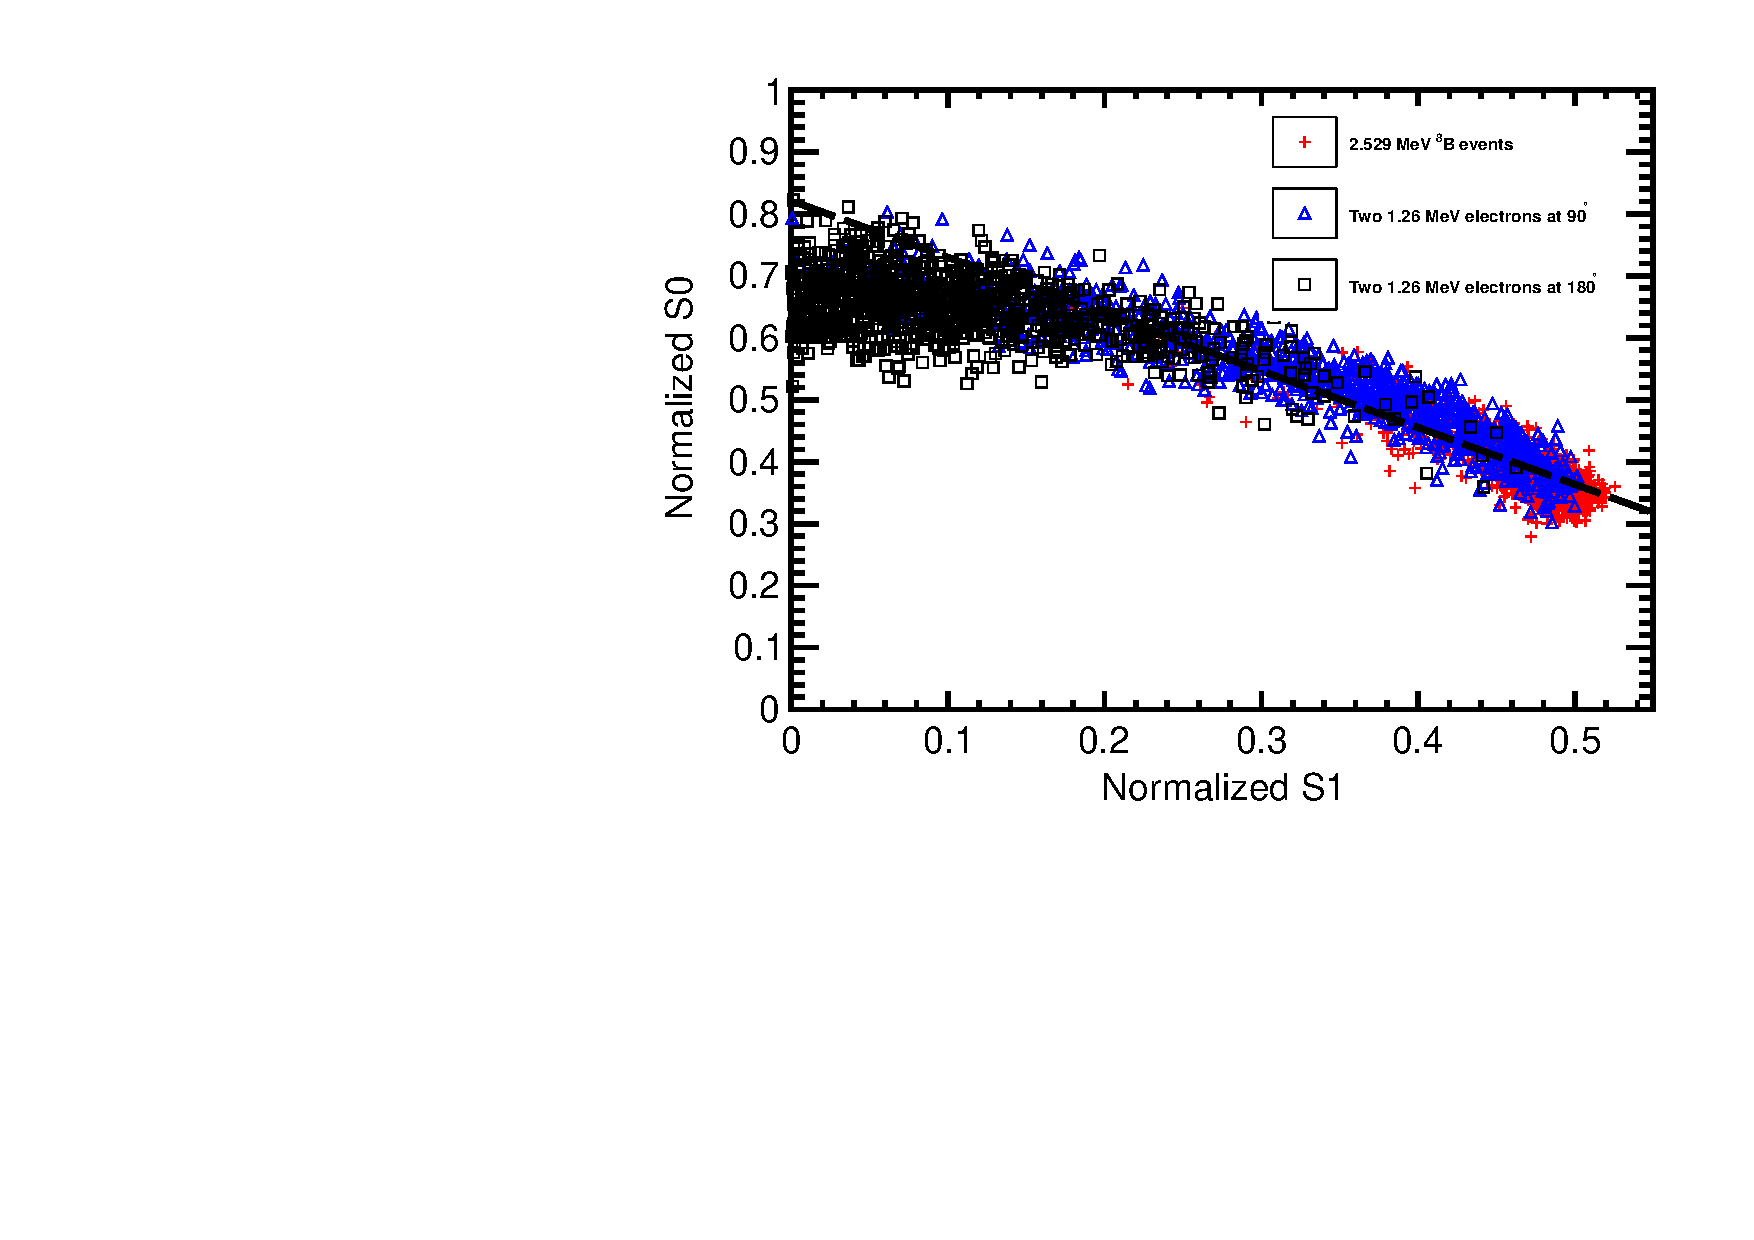
\includegraphics[width=0.49\textwidth]{ALL/hS0vsS1_topologies_CHELight_VtxSmear0cm_VtxShiftX0cm_33p5ns_center.pdf}
  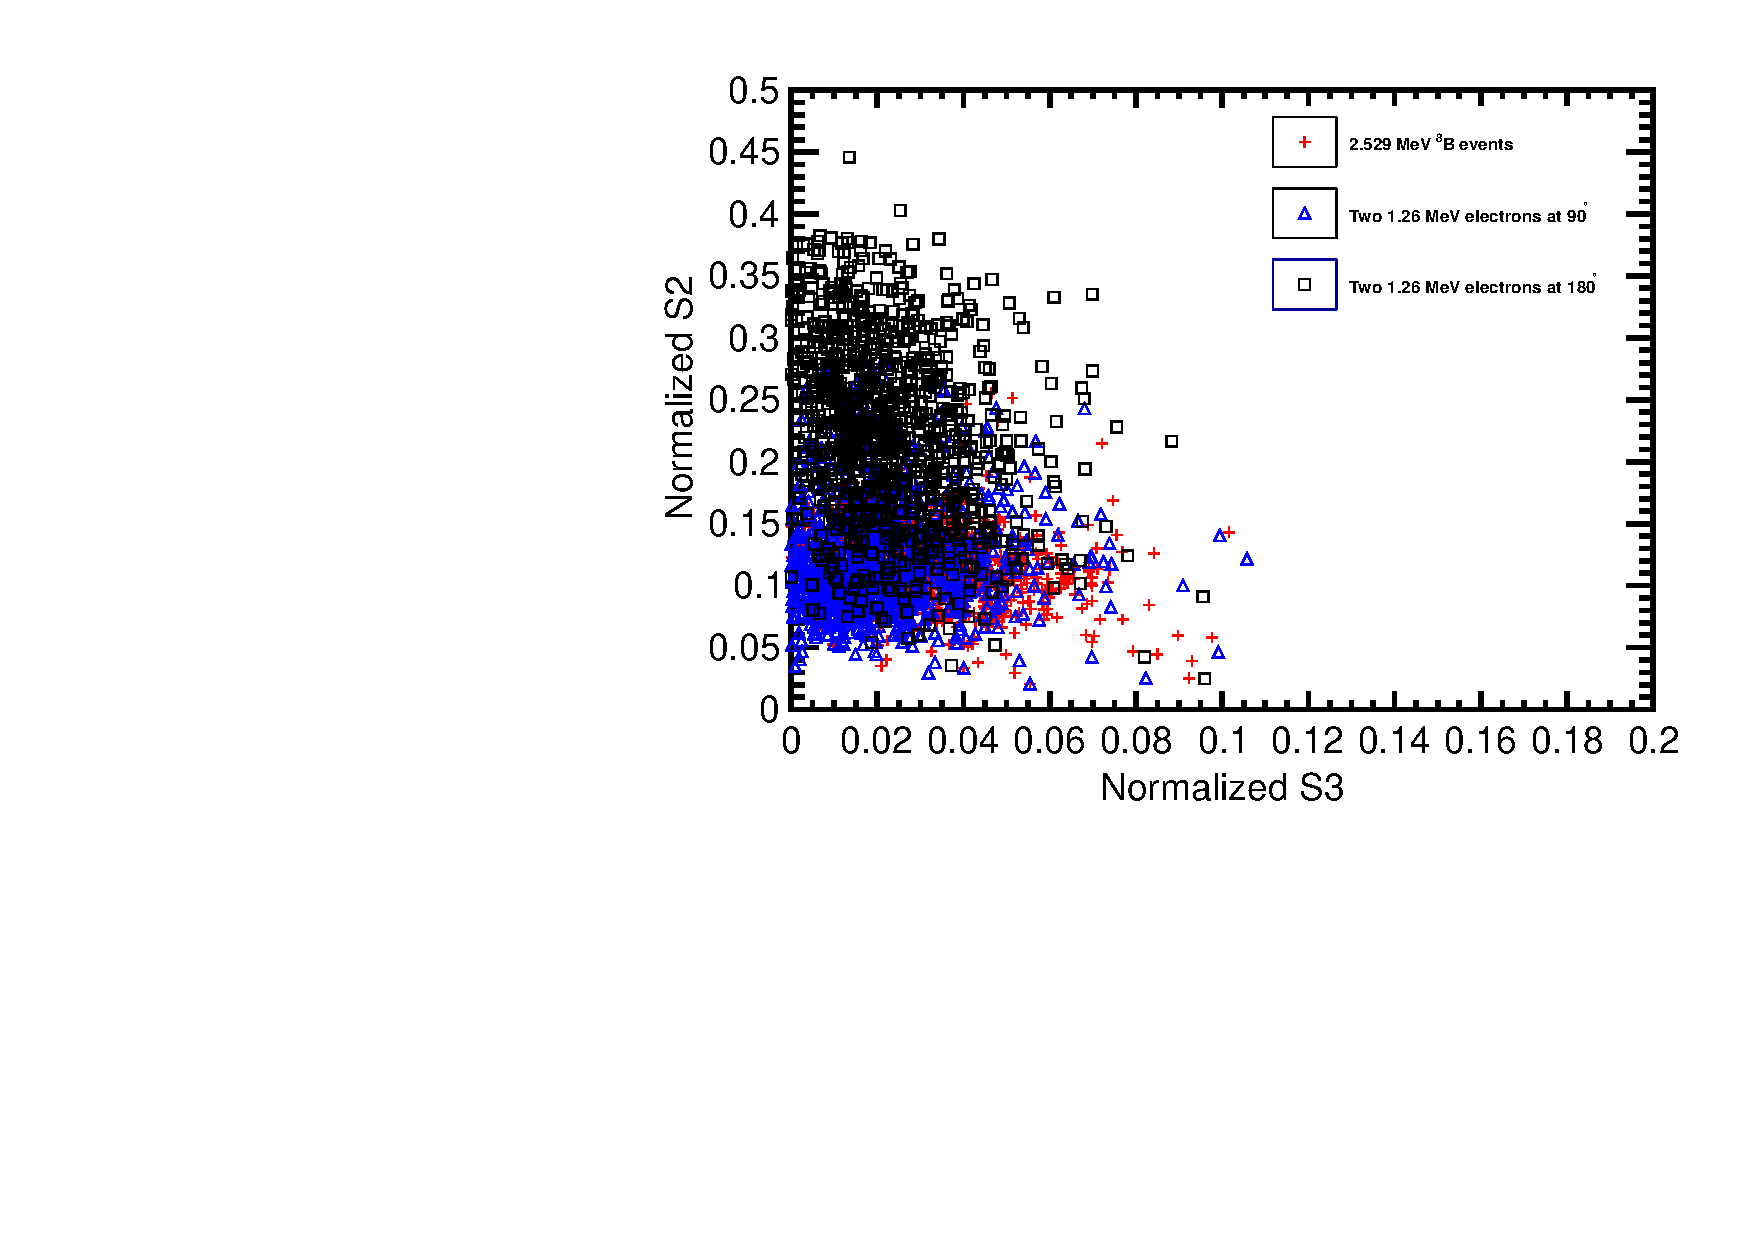
\includegraphics[width=0.49\textwidth]{ALL/hS2vsS3_topologies_CHELight_VtxSmear0cm_VtxShiftX0cm_33p5ns_center.pdf}
  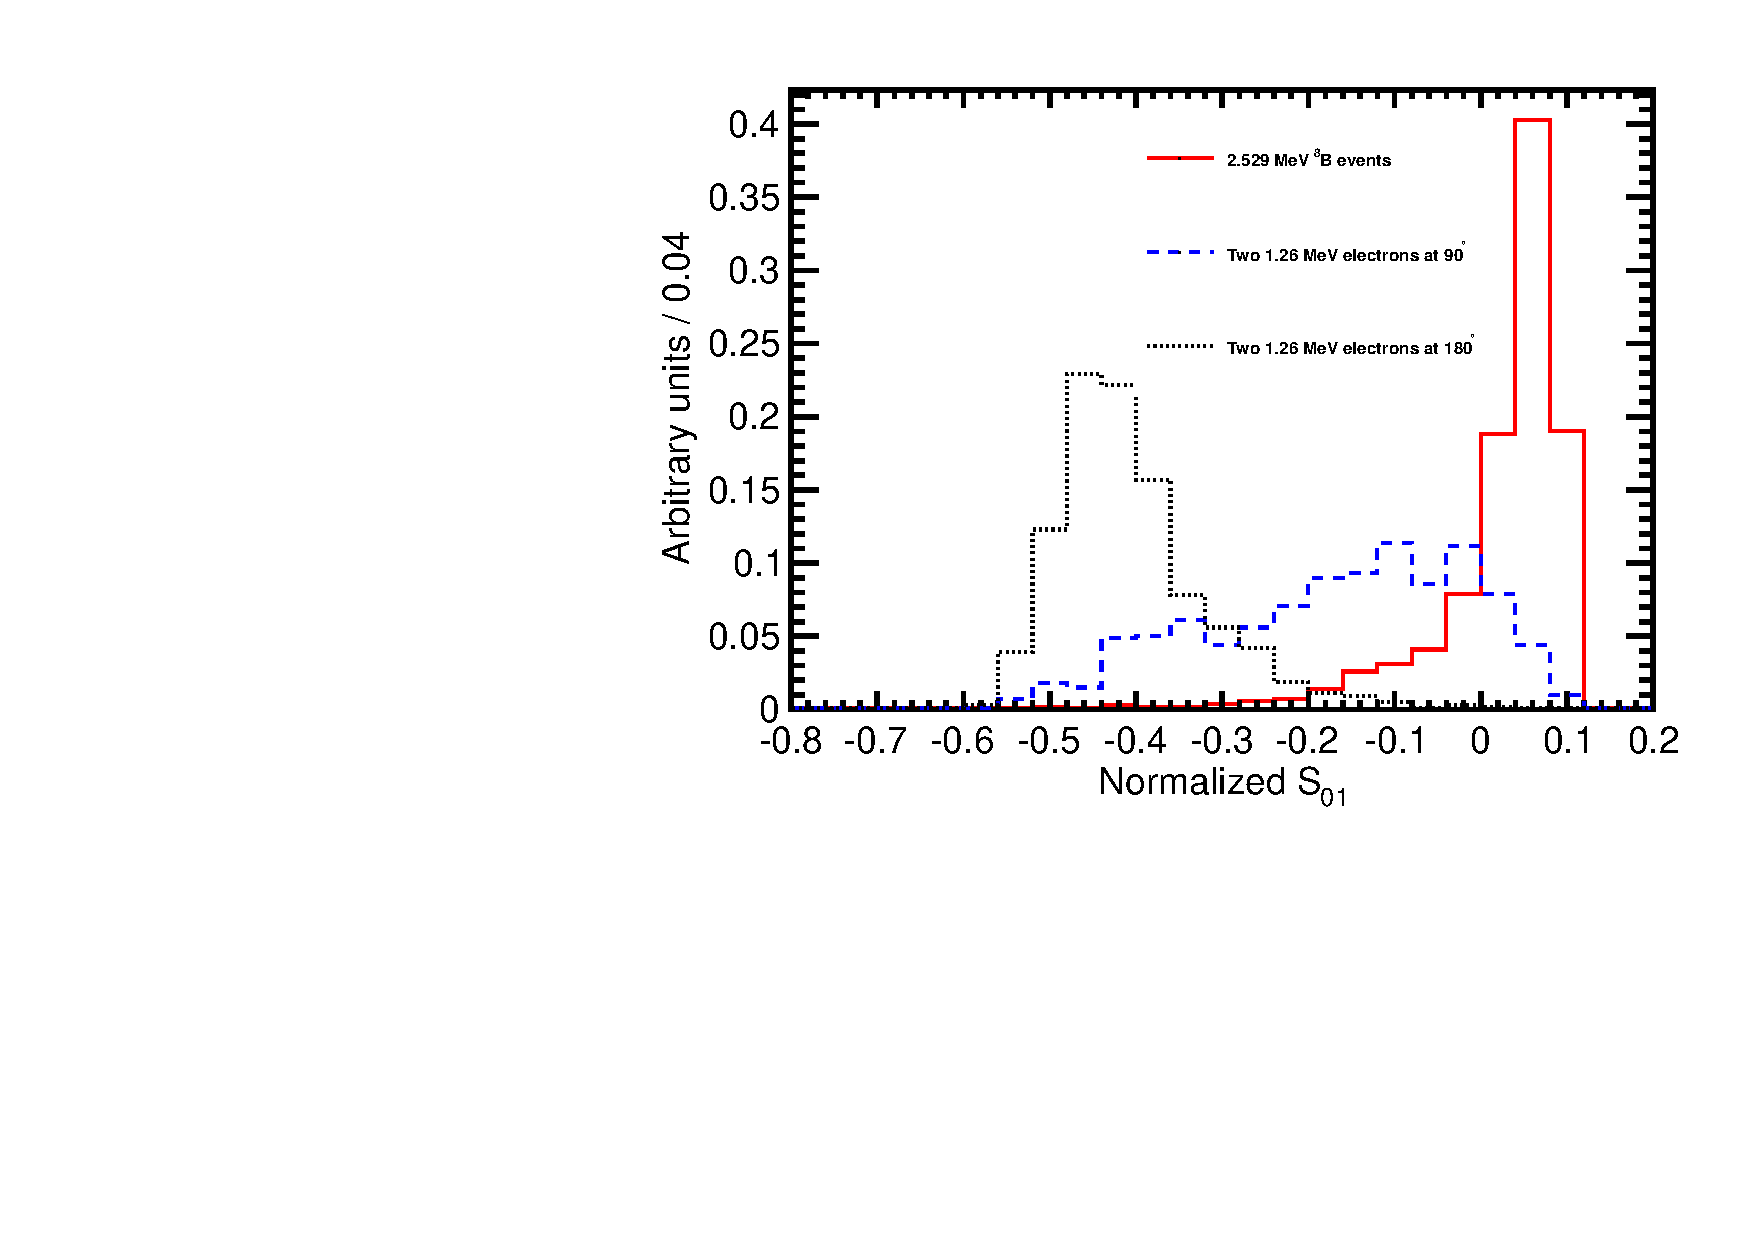
\includegraphics[width=0.9\textwidth]{ALL/hS01_topologies_CHELight_VtxSmear0cm_VtxShiftX0cm_33p5ns_center.pdf}
  \caption{Spherical harmonics for three event topologies: two
    back-to-back 1.26~MeV electrons (\emph{black squares and black
      dotted line}), two 1.26~MeV electrons at 90$^{\circ}$ angle
    (\emph{blue triangles and blue dashed line}), and a single
    2.529~MeV electron representing $^{8}$B background (\emph{red
      crosses and red solid line}). Simulation of 1000 events
    originated at the center of the sphere. Perfect separation between
    Cherenkov and scintillation light is implemented in this
    simulation by using only Cherenkov photons. \emph{Top left:} $S_0$
    versus $S_1$ scatter plot. Black dotted line is a linear fit of
    the 90$^{\circ}$ topology and $^{8}$B events. Variable $S_{01}$ is
    defined as a projection of 2D distribution onto this linear
    fit. \emph{Top right:} $S_2$ versus $S_3$ scatter
    plot. \emph{Bottom:} $S_{01}$ distributions for the three
    topologies. These distributions are normalized to unit area for
    shape comparison.}
  \label{fig:SL_topologies_CHE}
\end{figure*}


The effects due to the presence of scintillation light and applying the default QE are shown in Fig.~\ref{fig:SL_topologies_all}. Spherical harmonics of the same three representative event topologies are now calculated using early light (photons with arrival time less than 33.5~ns) that contains both directional Cherenkov light and uniform scintillation light. The of number PE seen by each tube is reduced by the default QE. In this more realistic scenario, the higher order multiple moments, S2 and S3, no longer provide noticeable separation between different event topologies.


\begin{figure*}[h]
  \centering
  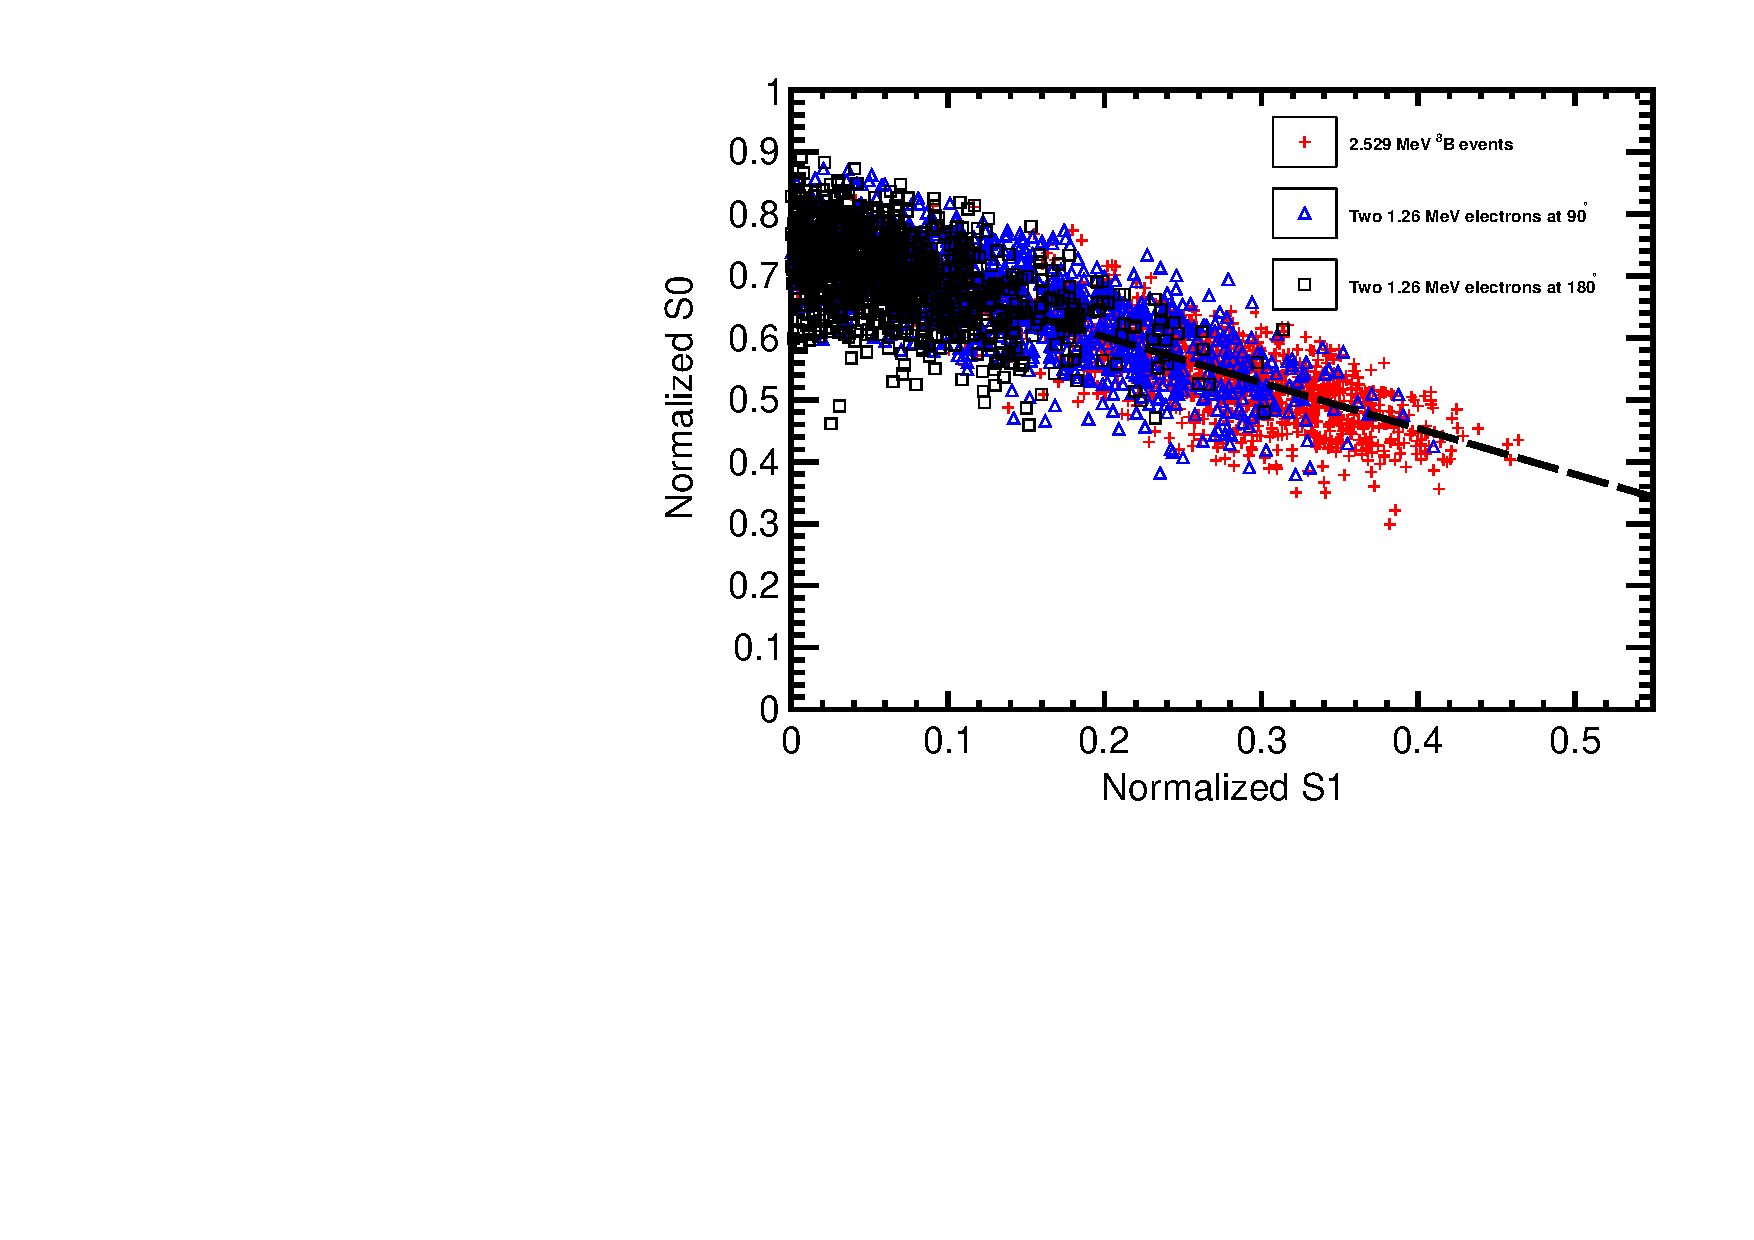
\includegraphics[width=0.49\textwidth]{hS0vsS1_topologies_allLight_VtxSmear0cm_VtxShiftX0cm_33p5ns_center.pdf}
  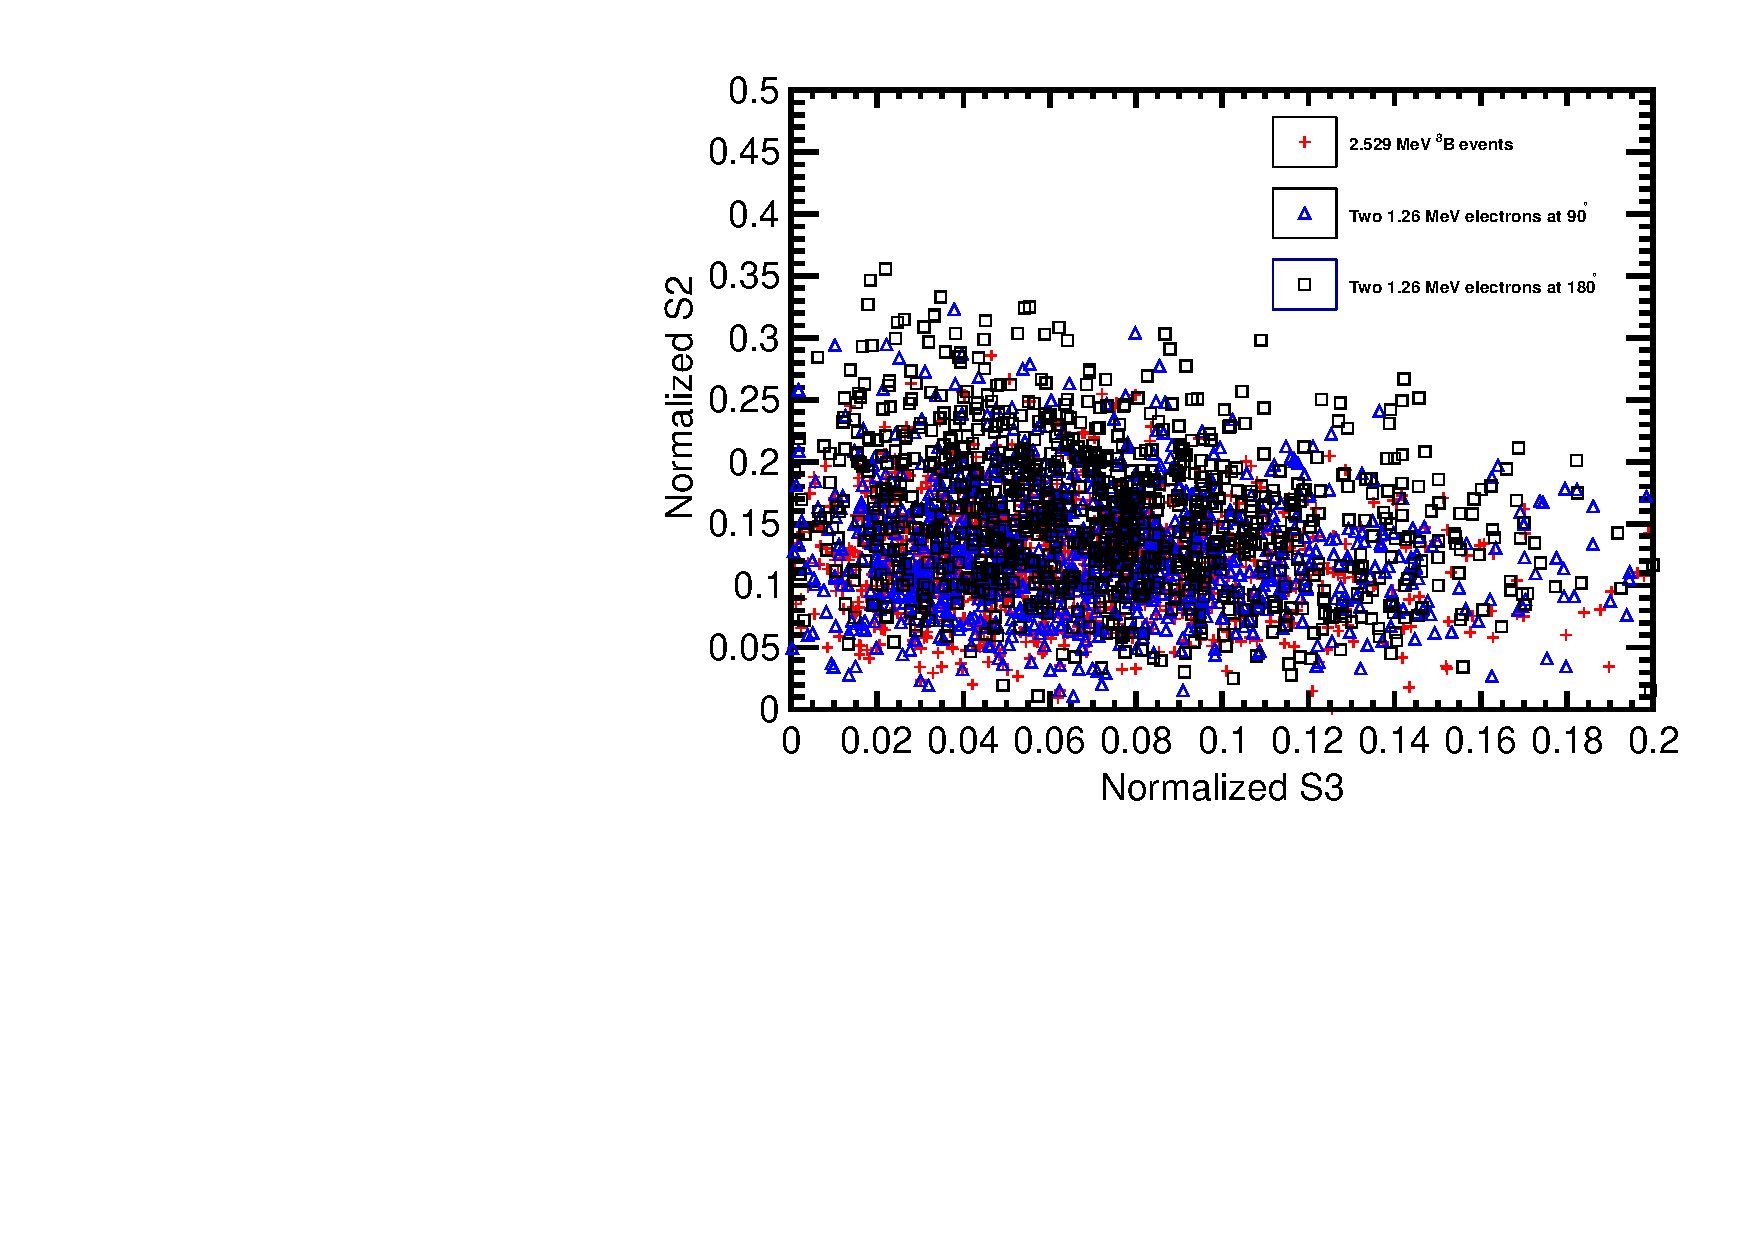
\includegraphics[width=0.49\textwidth]{hS2vsS3_topologies_allLight_VtxSmear0cm_VtxShiftX0cm_33p5ns_center.pdf}
  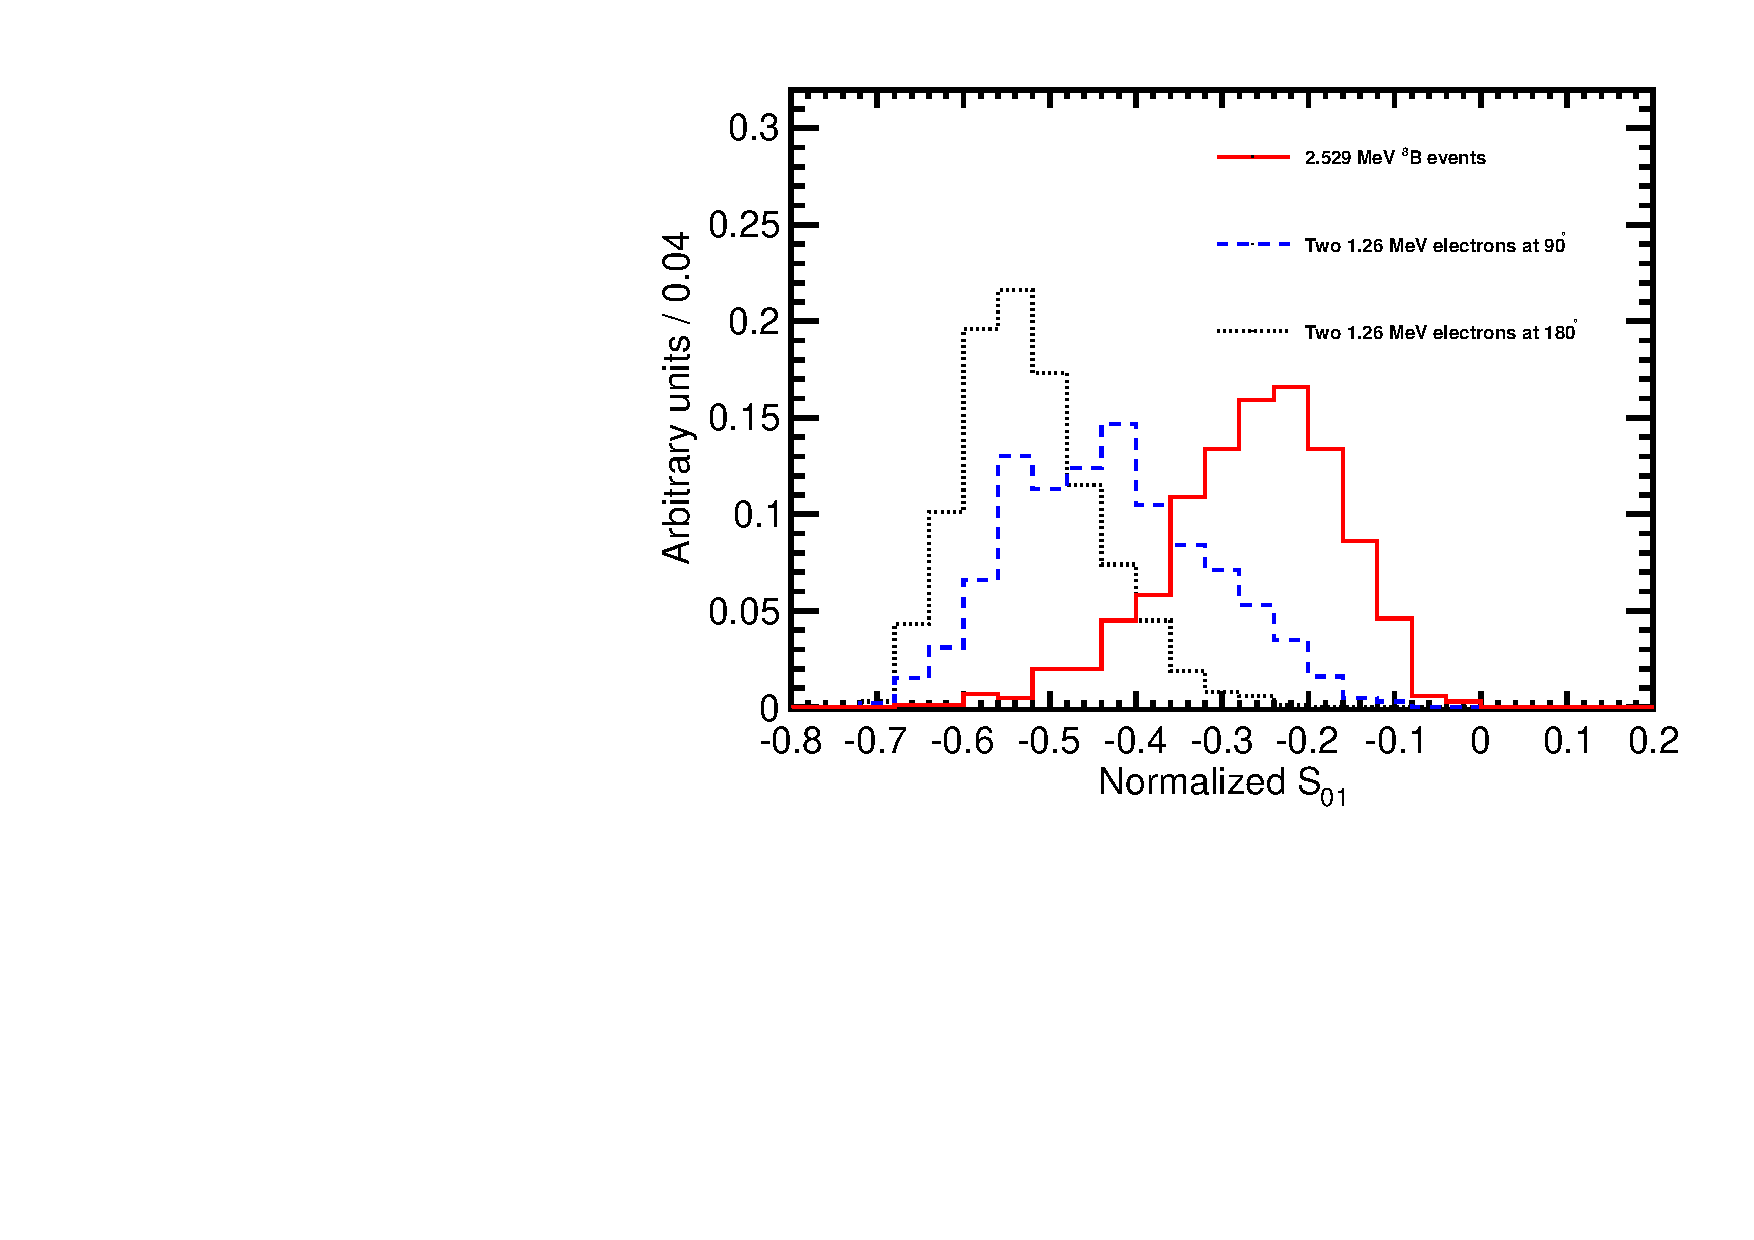
\includegraphics[width=0.9\textwidth]{hS01_topologies_allLight_VtxSmear0cm_VtxShiftX0cm_33p5ns_center.pdf}
  \caption{Spherical harmonics for three event topologies: two
    back-to-back 1.26~MeV electrons (\emph{black squares and black
      dotted line}), two 1.26~MeV electrons at 90$^{\circ}$ angle
    (\emph{blue triangles and blue dashed line}), and a single
    2.529~MeV electron representing $^{8}$B background (\emph{red
      crosses and red solid line}). Simulation of 1000 events
    originated at the center of the sphere. Separation between
    Cherenkov and scintillation light is implemented 33.5~ns cut on
    the photon arrival time. Perfect vertex reconstruction - true
    vertex position is used. \emph{Top left:} $S_0$ versus $S_1$
    scatter plot. Black dotted line is a linear fit of the
    90$^{\circ}$ topology and $^{8}$B events. Variable $S_{01}$ is
    defined as a projection of 2D distribution onto this linear
    fit. \emph{Top right:} $S_2$ versus $S_3$ scatter
    plot. \emph{Bottom:} $S_{01}$ distributions for the three
    topologies. These distributions are normalized to unit area for
    shape comparison}
\label{fig:SL_topologies_all}
\end{figure*}

